\documentclass[11pt]{article}

\usepackage[portuguese]{babel}
\usepackage[T1]{fontenc}
\usepackage[utf8]{inputenc}
\usepackage{amsmath}
\usepackage{graphicx}
\usepackage{subfig}
\usepackage[colorinlistoftodos]{todonotes}
\usepackage{listings}
\usepackage{color} 
\usepackage{float}
\usepackage[font={footnotesize}]{caption}
\usepackage{xcolor,colortbl}
\usepackage{array}
\usepackage{fixltx2e}
\setcounter{secnumdepth}{3}

\numberwithin{equation}{section}

\linespread{1.3}
\usepackage{indentfirst}
\usepackage[top=2.5cm, bottom=2.5cm, right=2.5cm, left=2.5cm]{geometry}



\begin{document}


\begin{titlepage}
	\begin{center}
		
		\hfill \break
		\hfill \break
		
		
\includegraphics[width=0.4\textwidth]{./logo}~\\[1cm]
		
		\textsc{\Large Mestrado Integrado em Engenharia Electrotécnica e de Computadores}\\[1.5cm]
		\textsc{\huge Sistemas Electrónicos de Processamento de Sinal}\\[0.4cm]
		
		{\huge \bfseries Desenvolvimento de um Modulador BPSK com uso de \textit{Costas Loop} \\[1.2cm]}
		
		Grupo n.º 3 \vspace{0.3cm}
		
		\begin{tabular}{l r}
			André Filipe Barroso Cerqueira \hspace{1mm} & n.º 65144 \\
			Guilherme Branco Teixeira \hspace{1mm} & n.º 70214  \\
			João André Catarino Pereira & n.º 73527
		\end{tabular}
		
		\hfill
		\hfill
		
		segunda-feira 15h30 - 18h30, LE1
		
	
		\vfill
		
		{\large Lisboa, 1 de Junho de 2015} 
		
	\end{center}
\end{titlepage}
\pagenumbering{gobble}
\clearpage

	\footnote{As linhas de código apresentadas durante o relatório têm como objectivo demonstrar a maneira de raciocinar na resolução de problemas, não representando uma cópia exata do código usado em laboratório, podendo até, serem consideradas \textit{pseudo-código}}
	
\tableofcontents
\pagebreak

\clearpage
\pagenumbering{arabic}

\section{Introdução}
O presente trabalho trata-se do projeto de laboratório da cadeira: desenvolvimento de um modem de $Binary$ $Phase$ $Shift$ $Keying$ (BPSK) usando um \textit{Costas Loop}. 

Teve como objectivo a familiarização com o ambiente de desenvolvimento integrado de DSP que consiste nas placas de desenvolvimento DSK TMS320C6416 e DSK TMS320C6713 da $Texas$ $Instruments$ e no software de desenvolvimento $Code Composer Studio v5.5$, e na implementação de alguns dos blocos de um modem BPSK, nomeadamente o \textit{Scrambler},  \textit{Differential coder and mapper}, \textit{Modulator} e \textit{Demodulator(Costas Loop)}.

No projeto foi utilizada a placa DSK TMS320C6713. Inicialmente, na primeira parte do projeto, foram estudados dois projetos exemplo (sine8\_buf e loop\_intr) e, usando as ferramentas de debug, alteraram-se certos parâmetros de forma a observar os efeitos nos sinais resultantes. Também se consolidaram os conhecimentos adquiridos desenvolvendo dois projetos: um oscilador sinusoidal controlado numericamente e um transmissor BPSK. 

Na segunda parte do projeto foram incluídos os dois blocos mencionados no desenvolvimento dos restantes, dimensionaram-se filtros e testou-se e analisou-se o dispositivo desenvolvido. Os projetos desenvolvidos foram incorporados nos anexos A, B e C podendo analisar os mesmos com maior detalhe.

\section{Projecto}

\subsection{Projectos de Demonstração}
Foram analisados dois projetos de demonstração com o intuito de familiarizar com os equipamentos e as principais rotinas do projeto.
\subsubsection{sine8\_buf}
\label{sec:sine8}
O objectivo deste projeto é representar a função sinusoidal, multiplicada por um determinado ganho, através de um conjunto de amostras que equivalem a um período da mesma, repetindo nos períodos seguintes esse mesmo conjunto. Este procedimento é realizado através da rotina de interrupção presente no programa. 

Ao analisar o código deste projeto, à primeira vista podemos concluir logo que este usa uma frequência de amostragem de 8 kHz , tem um ganho $G=10$ predefinido e usa 8 amostras para representar a sinusoide. Depois de observar a sinusoide no osciloscópio variou-se o ganho a fim de perceber a sua influência e também o seu limite.
 
Para compreender o limite desta sinusoide é necessário ter em conta que se usa o formato de vírgula fixa Q15 para as suas amostras. Este formato tem como limite o valor $(2^{15}-1) = 32767$. Considerando o valor máximo da sinusoide, se multiplicarmos a mesma por um ganho $G=33$ obtemos um valor superior ao permitido pelo formato Q15 (\textit{overflow}), fazendo com que nesses pontos o valor da sinusoide seja o inverso do que deveria ser, ou seja ocorre \textit{wraparound} na variável da sinusóide (como se poderia esperar dado que se programa em C).   

\subsubsection{loop\_intr}
\label{sec:loop}
Este projeto fornece-nos um template para os próximos projetos, em termos de comunicação com a placa e rotina de interrupção. Pode-se observar nas últimas linhas de código como se liga os sinais de entrada e saída aos canais da placa.
                                         
No projeto anterior observou-se os efeitos de \textit{overflow} de uma variável. Neste observam-se os efeitos de aliasing  devido ao sinal de line-in ter a mesma frequência que a frequência de amostragem. A partir dos 4kHz deixamos de ver uma sinusoide com os 3.3V. Não foi feita a experiência de mudar para sinal quadrado e variar a frequência, mas provavelmente não se iria ver um sinal quadrado porque o espectro (infinito) deste teria que ser filtrado pelo anti-aliasing filter. 

\subsection{BPSK Modem}
Este projeto é constituído por duas partes, a primeira é um oscilador controlado numericamente e a segunda é um transmissor BPSK. Devido à existência de um inversor na placa utilizada deu-se, ao longo deste projeto, atenção ao efeito do inversor nos sinais, como se poderá observar nas próximas secções.

\subsubsection{P1. Oscilador controlado numericamente}
\label{NCO}
Usou-se o projeto descrito na secção \ref{sec:loop} como base para a construção de um oscilador controlado numericamente (\textit{NCO}). Um \textit{NCO} é um gerador de sinal digital que cria uma forma de onda discretamente representada no tempo e na amplitude. O \textit{NCO} tem as seguintes características:

\begin{table}[H]
	\centering
	\caption{Características do \textit{NCO} a construir.}
	\label{tab:NCO-car}
\begin{tabular}[c]{|l||c|c|}
	\hline \textbf{Parâmetro} & \textbf{Símbolo} & \textbf{Valor} \\ 
	\hline Frequência de amostragem & $ f_{s} $ & $ 16 kHz $ \\ 
	\hline Frequência mínima & $ f_{min} $ & $ 2 kHz $ \\ 
	\hline Frequência máxima & $ f_{max} $ & $ 6 kHz $ \\ 
	\hline
\end{tabular}
\end{table}

O projeto de construir o \textit{NCO} seguiu os seguintes passos que estão posteriormente explicados:

\begin{enumerate}
	\item Oscilador de Relaxação (Integrador de Rampa). 
	\item Look-up-table (LUT). 
	\item Obtenção de um sinal sinusoidal através da LUT.
	\item Criação de variáveis para controlo da frequência e amplitude do sinal sinusoidal.
	\item Utilização do sinal de entrada para controlar a frequência do sinal.
	\item Teste do oscilador com uma onda sinusoidal à entrada.
	\item Melhoria da qualidade do oscilador com interpolação linear.  
	\item Comparação dos espectros com e sem interpolação.
\end{enumerate}
%\pagebreak

\paragraph{1.Oscilador de Relaxação} \hspace{0pt}
\label{p1-1}

Para construir um Oscilador de Relaxação foi criada uma rotina que, em cada ciclo, incrementa a variável de amplitude do sinal de saída de modo a que este tenha o comportamento de uma rampa. Para que esta tenha precisão máxima e amplitude máxima de 1 V foi usado o formato Q15 para representar o sinal de saída, pois este formato tem amplitude máxima de $2^{15}-1 = 32767 $.

Tendo em conta as frequências da tabela \ref{tab:NCO-car}, podemos chegar aos seguintes valores de incremento com as suas frequências correspondentes.                      
\begin{table}[H]
	\centering
	\caption{Valores a atribuir ao incremento do sinal na saída.}
	\label{tab:incrementos}
	\begin{tabular}[c]{|l||c|}
		\hline \textbf{Frequência de saída($f_0$)} & \textbf{Incremento($\Delta$)}\\ 
		\hline $ 2 kHz \quad (f_{min}) $ & $ 8192 $\\ 
		\hline $ 4 kHz $ & $ 16384 $  \\ 
		\hline $ 6 kHz \quad (f_{max}) $ & $ 24576 $ \\ 
		\hline
	\end{tabular}
\end{table}
Os valores na tabela \ref{tab:incrementos} foram calculados através da seguinte fórmula:
\begin{equation}
 f_{0}= \frac{\Delta}{2A}f_{s} \Leftrightarrow \Delta= 2A\frac{f_{0}}{f_{s}} \hspace{3 mm}, A=32767
\end{equation}
Esta equação trata-se de determinar quantos incrementos se faz de -32767 a 32767 ($2A$), de modo a que ocorra \textit{wraparound}, sabendo que em cada ciclo da frequência de amostragem $T_s=\frac{1}{f_s}$ se faz um incremento $\Delta$ para se ter um período de rampa $T_0=\frac{1}{f_0}$.

Foi então possível obter as seguintes rampas com diferentes frequências:
\begin{figure}[H]
	\centering
	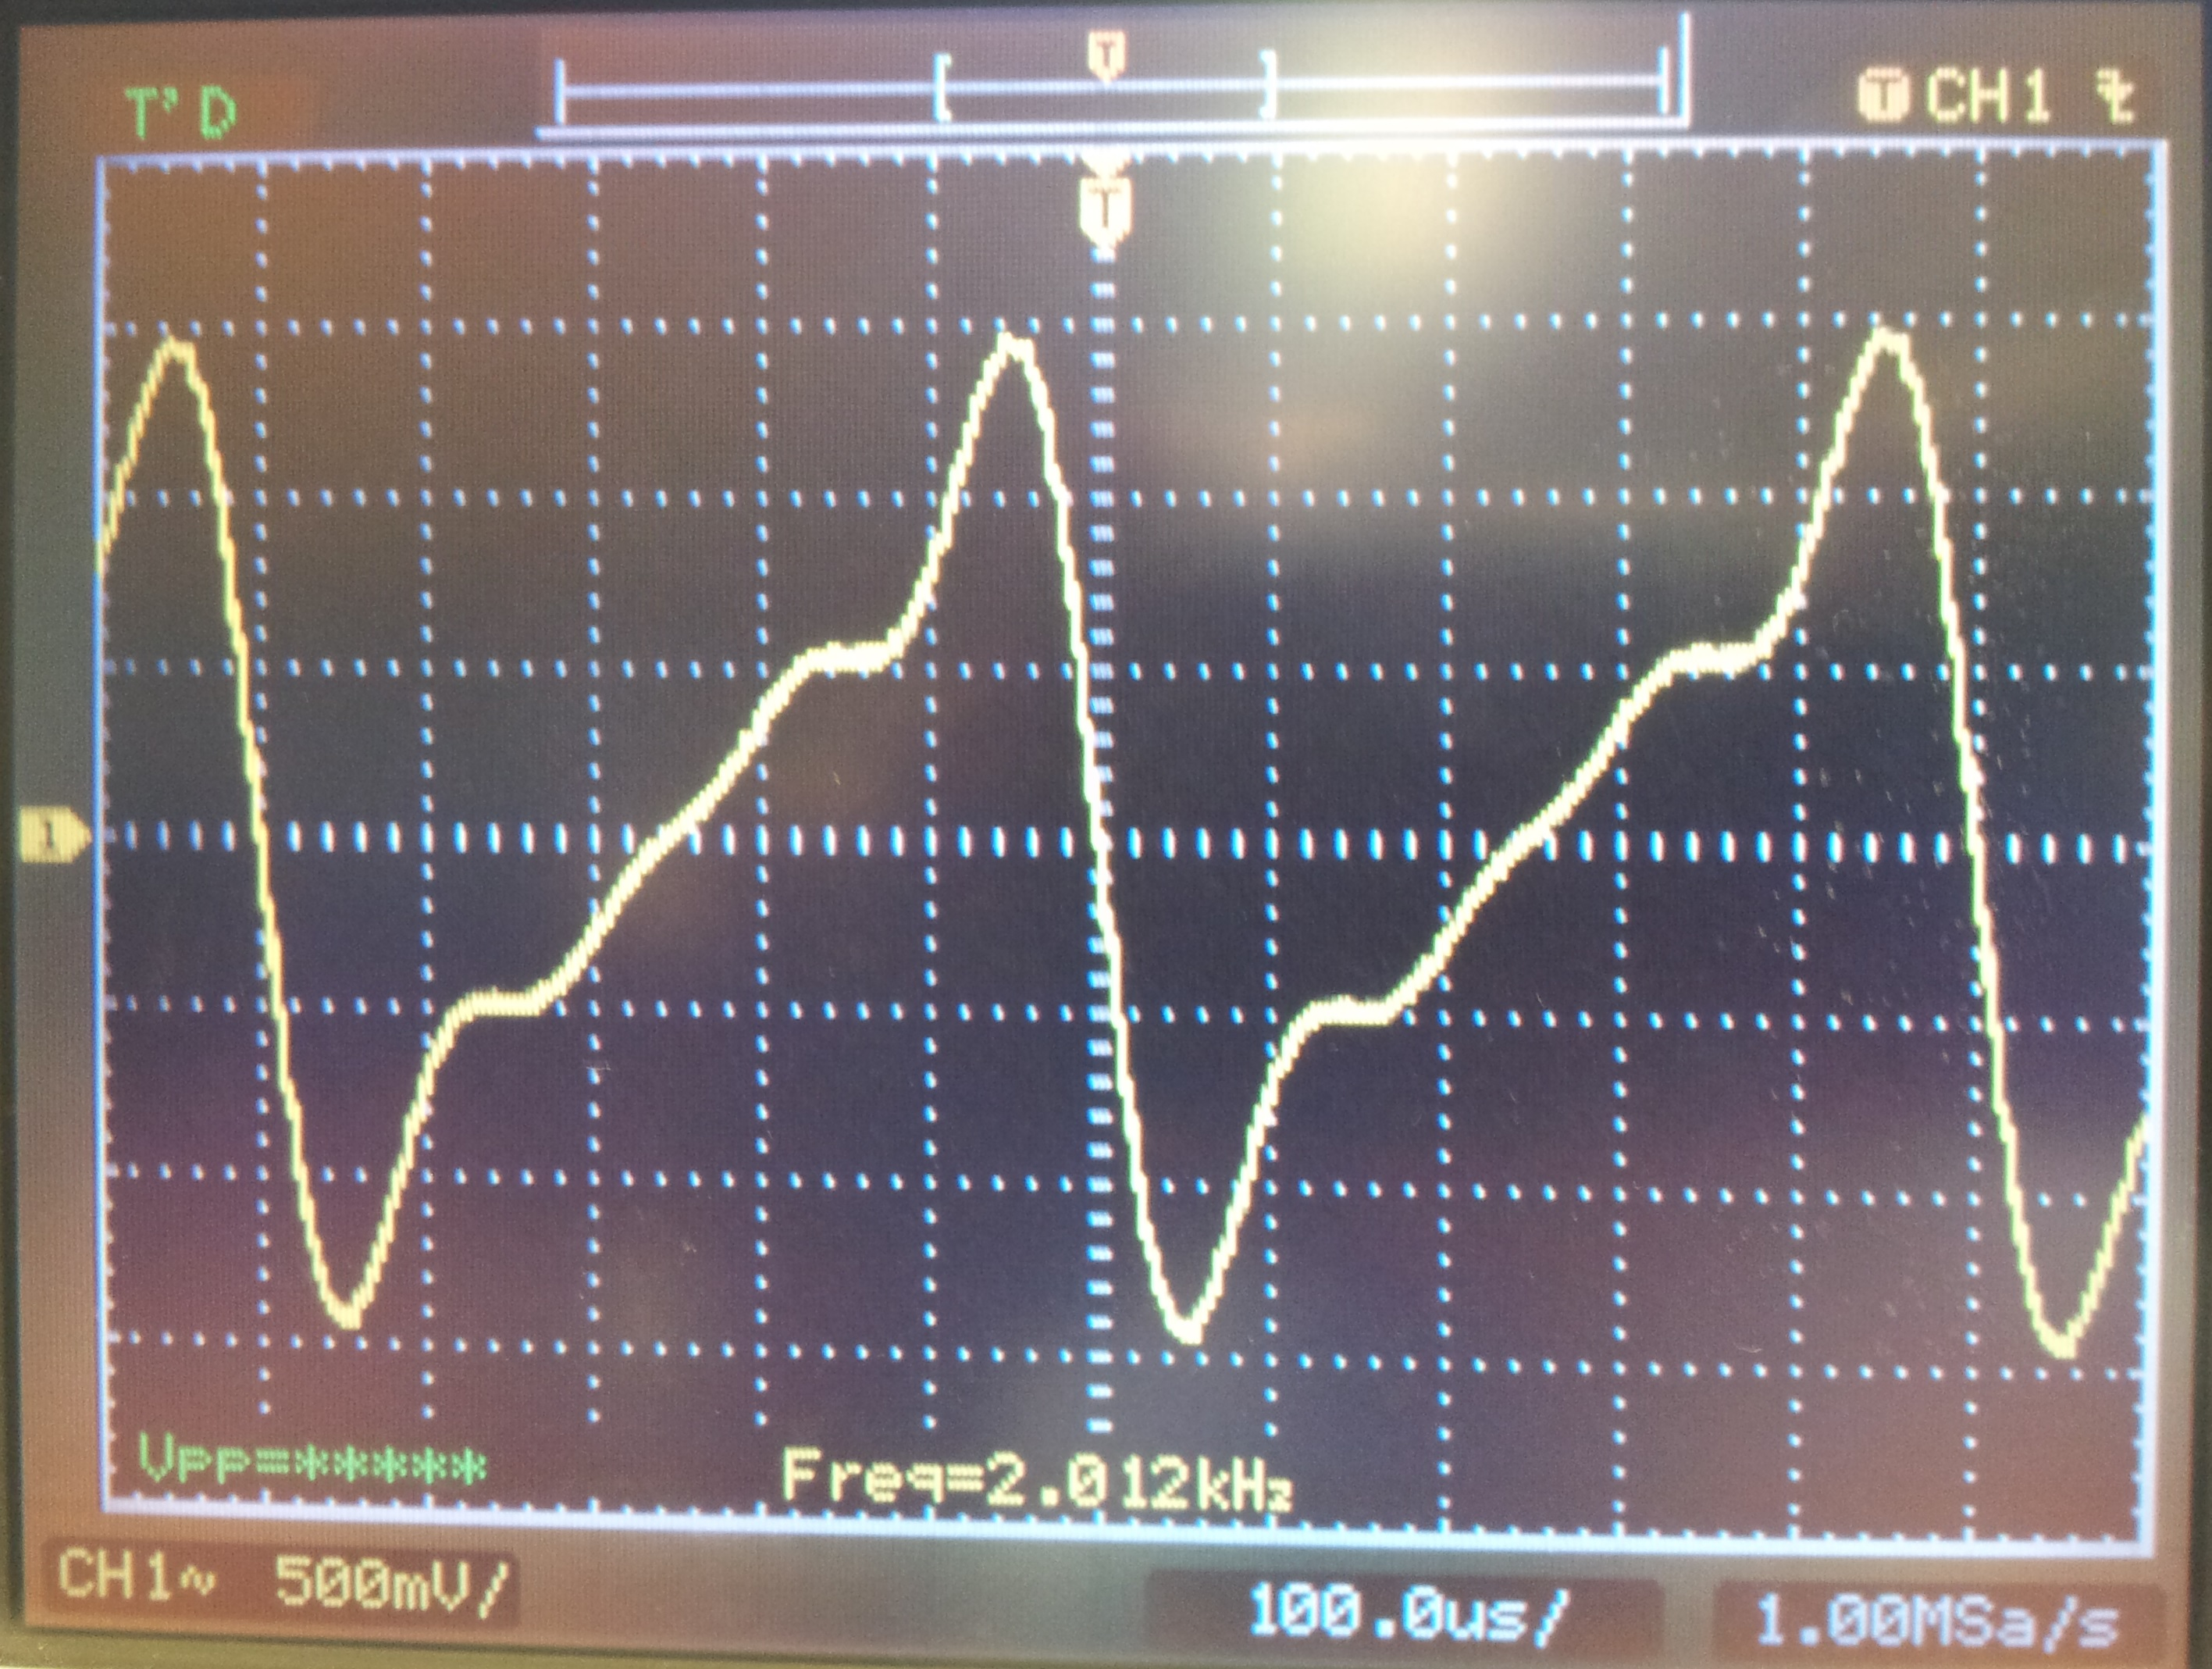
\includegraphics[width=0.5\textwidth]{./P1_2kHz}~\\
	\caption{Rampa com frequência de $ 2 kHz $}
\end{figure}

\begin{figure}[H]
	\centering
	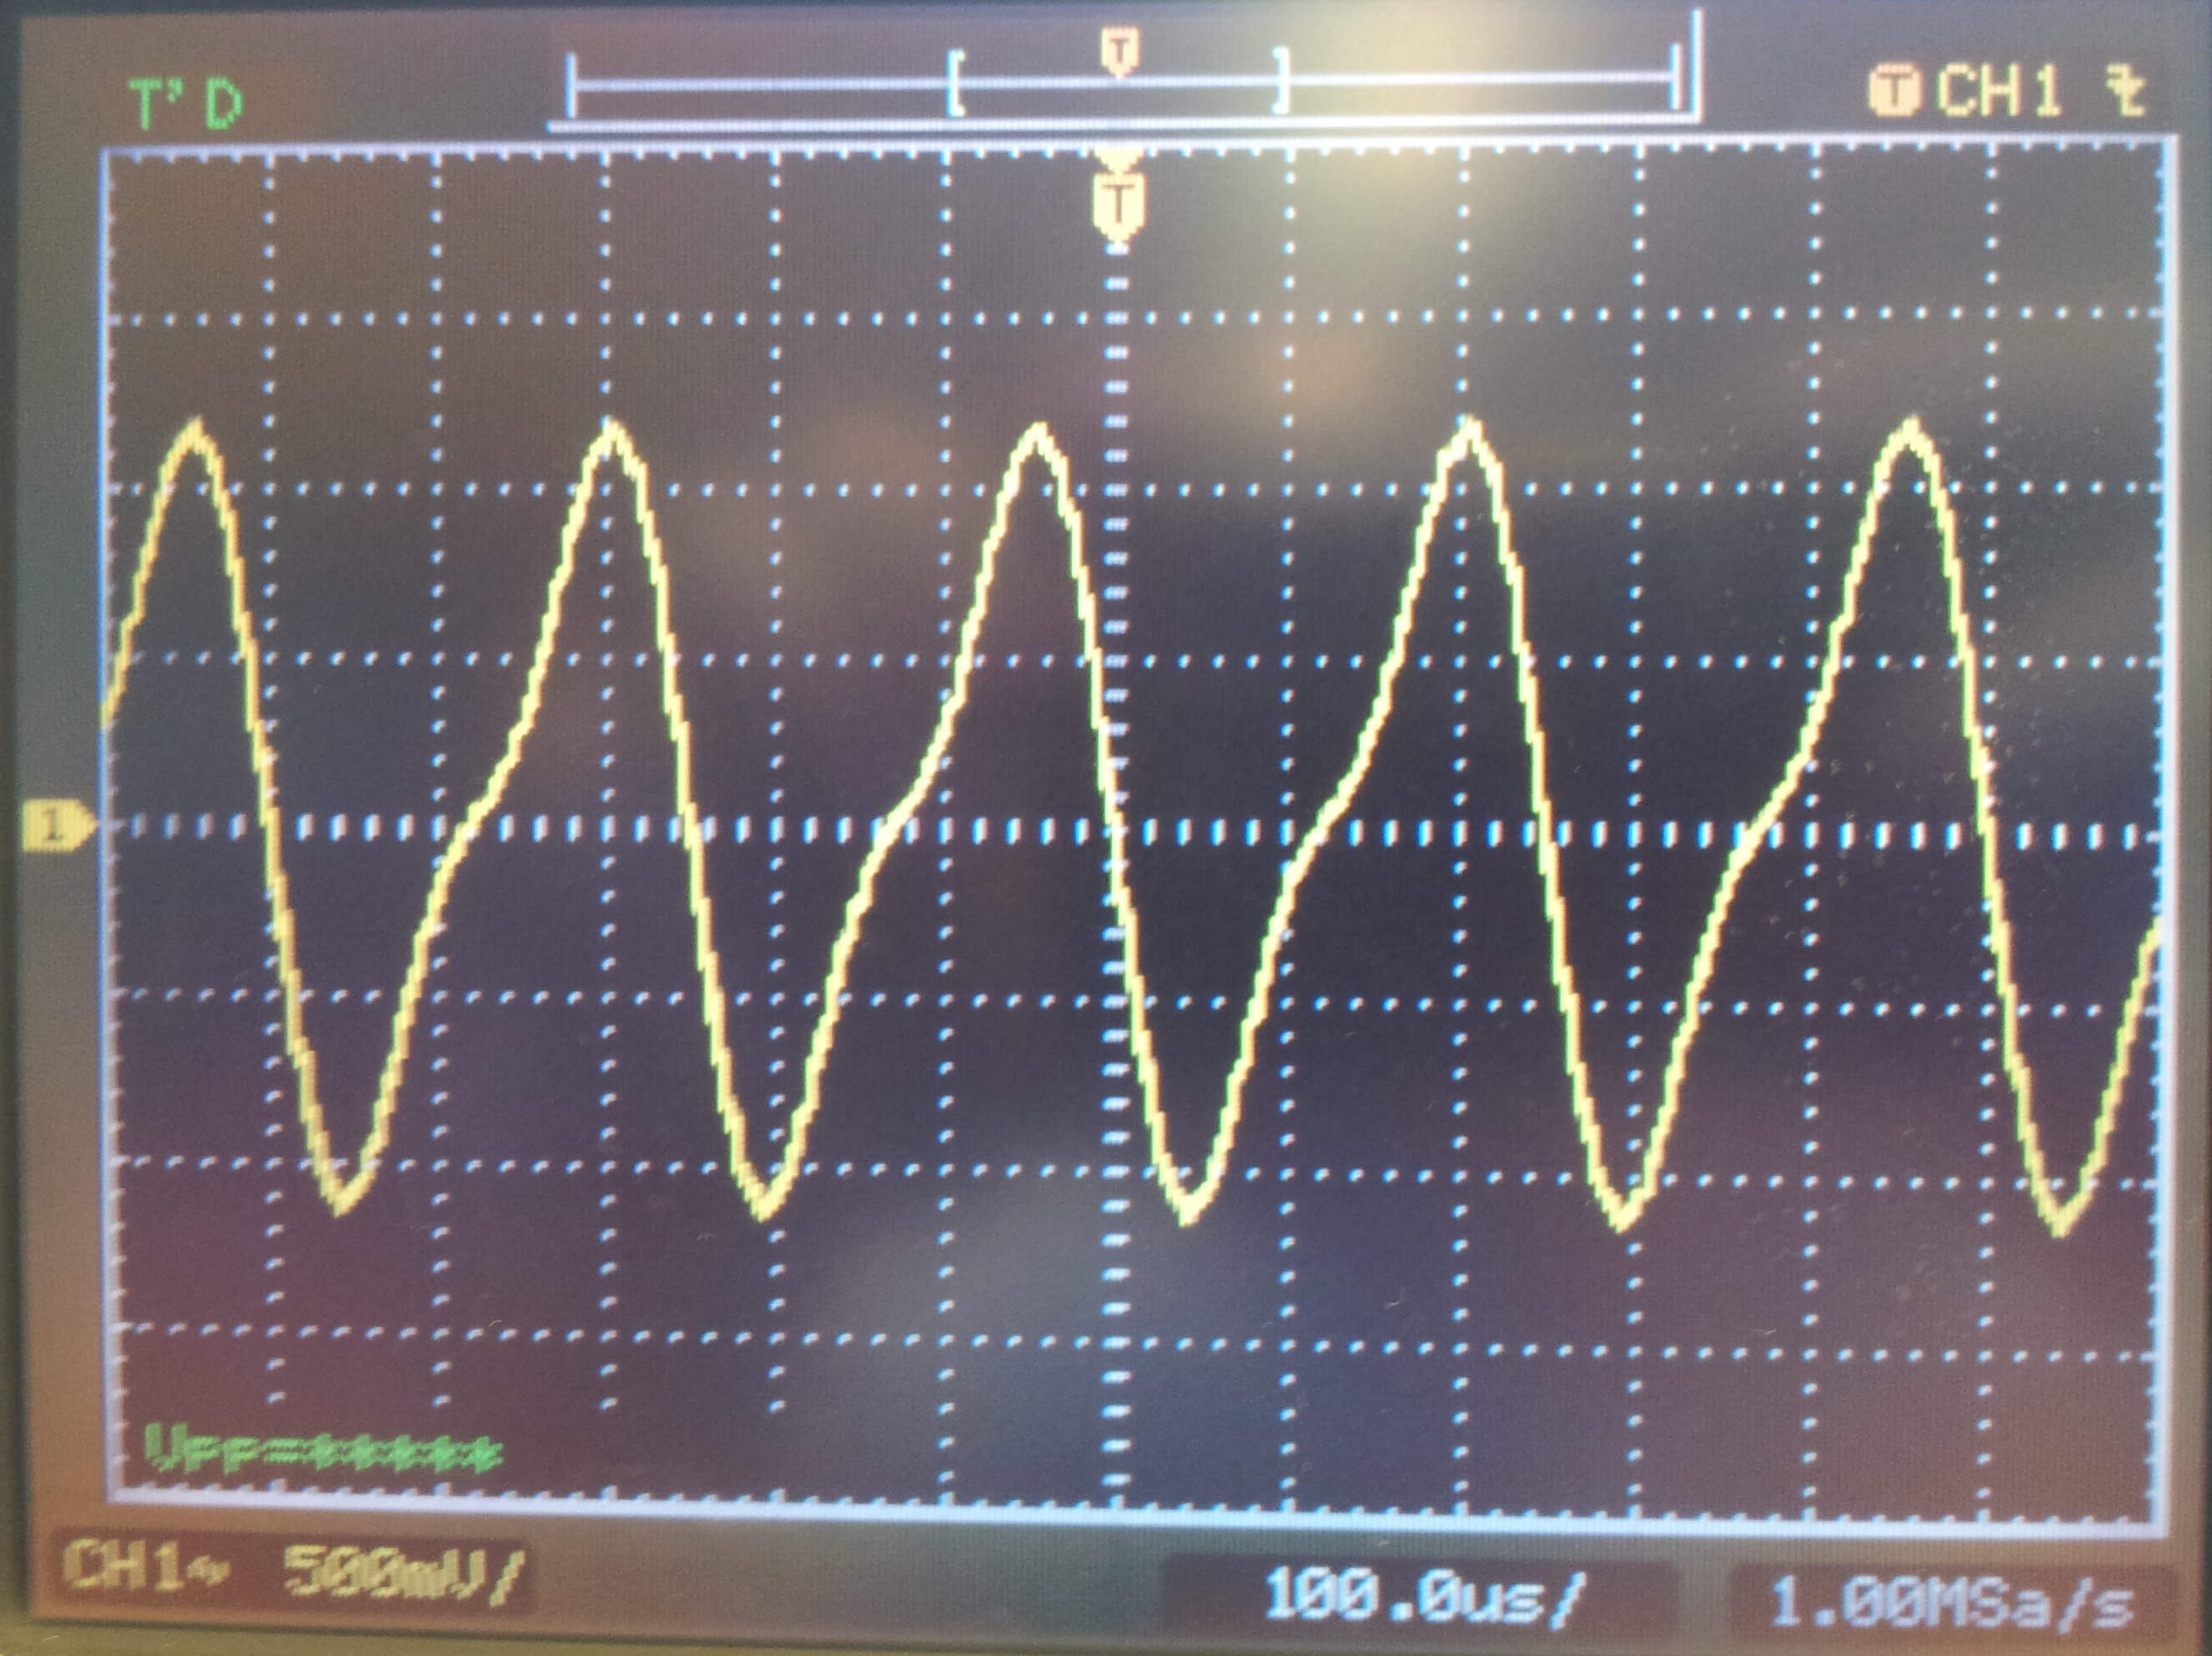
\includegraphics[width=0.5\textwidth]{./P1_4kHz}~\\
	\caption{Rampa com frequência de $ 4 kHz $}
\end{figure}

Ao observar as duas rampas pode-se constatar que para uma frequência mais baixa, ou seja, um incremento menor, a rampa apresenta mais "degraus" e um menor declive. Um incremento menor na rampa significa um maior número de amostras da mesma dentro do intervalo possível, o que reduz o declive da rampa. É de salientar que devido à presença do inversor da placa foi introduzido o simétrico da rampa calculada no canal de modo a observar esta no sentido correto.
\paragraph{2.\textit{Look-up-table}} \hspace{0pt}
\label{p1-2}

Foi criada uma tabela (LUT) com os valores em Q15 de meio ciclo de um seno de modo a que seja possível retirar os seus valores para criar um sinal sinusoidal. Esta tabela tem 32 valores e foi construída com a seguinte equação:
\begin{equation}
round \left(32767*\sin \dfrac{n \pi}{32} \right),  \quad \quad n=0,1,2,...,31
\end{equation}

Para calcular apenas meio ciclo do seno, é necessário ter 32 valores pertencentes ao intervalo $[0,\pi]$ na fase. Assim, é necessário restringir a fase a esse intervalo através da divisão observada na expressão, $\frac{n \pi}{32}$. O produto do seno pelo valor 32767 é a conversão do seno para Q15. 

Não se multiplica por $2 ^{15}=32768$ pois os sinais estão em complemento para dois, o que significa que, para o máximo do seno, esta LUT ultrapassaria o limite do formato, o que causaria \textit{overflow} nessa amostra do sinal resultando num sinal incorreto.

Como a tabela LUT inclui apenas meio ciclo de seno, ao criar a sinusoide é necessário negar os valores adquiridos ao criar o segundo meio ciclo do seno.

\paragraph{3.Obtenção de um sinal sinusoidal através da LUT} \hspace{0pt}
\label{p1-3}

Usando como base a rampa criada na secção P1-1 para indexação da LUT criada na secção \ref{p1-2}, foi possível criar um sinal  sinusoidal.
                                                      
De acordo com o projeto, a rampa é representada num formato Q10, com 1 bit sinal, 5 bits inteiros e 10 bits fraccionários. 
Para a indexação são usados os 5 bits inteiros, ou seja, os 5 mais significativos (excluindo o bit de sinal) do sinal da rampa. Esses 5 bits irão apontar para o valor da tabela de LUT a usar para criar a sinusóide. 
Este processo foi efetuado com o seguinte pedaço de código dentro do ciclo:
\begin{lstlisting}
	rampa=rampa+delta;    //Criar a rampa
	index=rampa>>10;
	index=31 & index;         //Usar apenas 5 bits
	sinusoide=LUT[index];
\end{lstlisting}

Como se pode ver, para isolar os 5 bits inteiros fez-se dez \textit{shifts} para a direita de maneira a ter um sinal apenas com zeros, o bit sinal e esses 5 bits encostados à direita. A seguir aplicou-se uma máscara constituída por uma AND com 31 bits, de maneira a retirar o bit sinal e finalmente isolar num sinal o índice pretendido da LUT. Com o índice é uma questão de aceder à tabela e obter \textit{y1}, neste caso representado pelo sinal \textit{sinusoide} (Figura \ref{fig:sen2k}).
\begin{figure}[H]
	\centering
	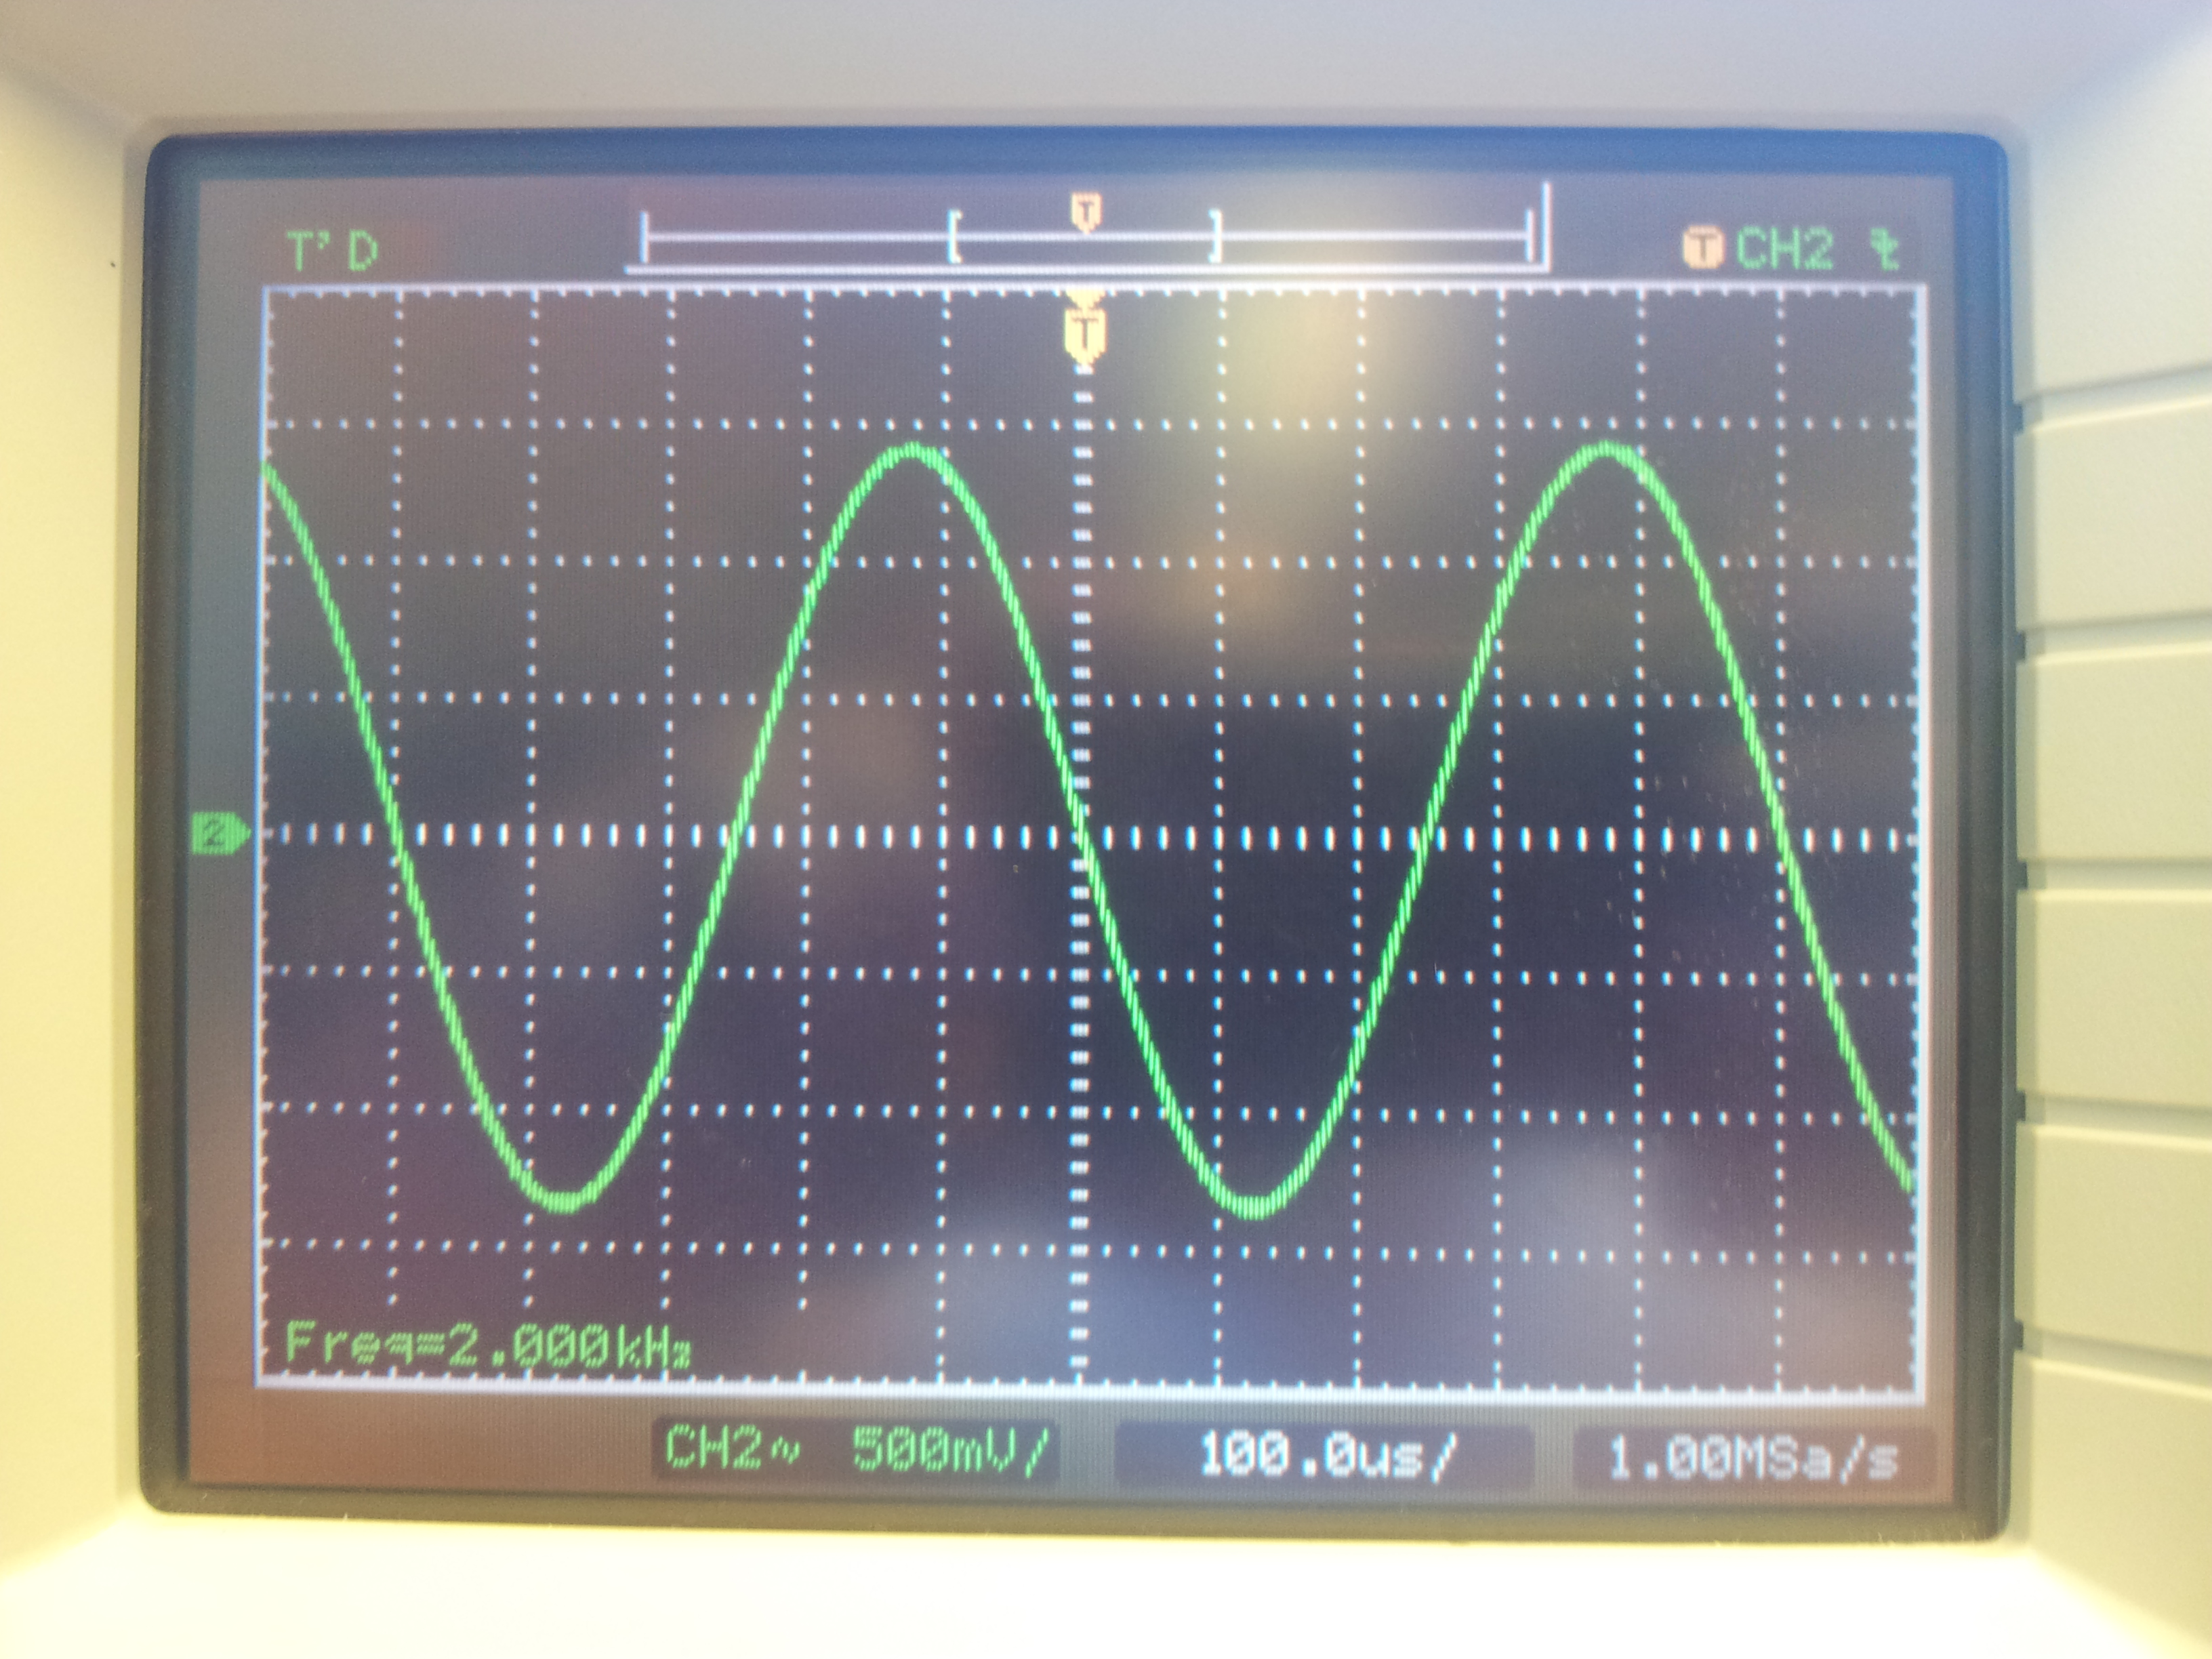
\includegraphics[width=0.5\textwidth]{./P1_1seno}~\\
	\caption{Sinal sinusoidal criado de $ 2 kHz $.}
	\label{fig:sen2k}
\end{figure}

Como se pode observar na figura foi possível criar um sinal aproximadamente sinusoidal através de uma LUT indexada por uma rampa. Nesta figura não é possível notar mas quando se aproxima mais o sinal no osciloscópio verifica-se pequenos degraus ao longo do sinal, que simbolizam a aproximação obtida através das amostras.

\paragraph{4.Criação de variáveis para controlo da frequência e amplitude do sinal sinusoidal} \hspace{0pt}
\label{p1-4}

Foram criadas duas variáveis para que fosse possível controlar a frequência e a amplitude do sinal à saída, \textit{delta} e \textit{ampl}, respectivamente.

A primeira variável foi já antes referida, nas secções \ref{p1-1} e \ref{p1-3}. Esta variável, caso alterada iria alterar a frequência da rampa, e por consequência, a frequência do sinal de saída. Como se pode observar na tabela \ref{tab:incrementos}, esta variável terá como limite máximo o valor $ 24576 $ e como limite mínimo $ 8192 $ devido às frequências mínima e máxima. Podemos também concluir que quanto maior for esta variável, maior a frequência do sinal de saída e também se o seu valor diminuir, a frequência de saída irá diminuir.

A segunda variável (\textit{ampl}) foi criada com o propósito de modelar a amplitude do sinal de saída. Esta causou mudanças mais significativas no código, tal como se pode verificar:
\begin{lstlisting}
	rampa=rampa+delta;
	index=rampa>>10;
	index=31 & index;        
	aux=ampl*LUT[index];
	aux=aux<<1;            //Retirar bit de sinal extra
	sinusoide=-aux>>16;    //Colocar o sinal com 16 bits em Q15
\end{lstlisting}

Esta variável tem como valor máximo $ 32767 $, pois os valores afixados na tabela LUT já apresentam um valor com a amplitude máxima de Q15 de maneira a não ter problemas com o formato de representação nem com a amplitude do sinal transmitido à placa.
Como se pode ver no código a variável \textit{ampl} multiplica diretamente pela LUT. 
\vspace{2 mm}

Quando se multiplica dois sinais, o sinal resultante fica com um bit sinal replicado que é eliminado através de um \textit{shift} esquerdo. Mas depois ainda é necessário ir buscar os 16 bits mais significativos através de 16 \textit{shifts} para a direita pois pretende-se um sinal com 16 bits em Q15. 

Na equação seguinte pode-se observar como obter o formato resultante num produto:
\begin{equation}
Q_{m} * Q_{k}=Q_{m+k-n+1}
\end{equation}

Neste caso como se multiplica dois sinais Q15 e \textit{n}$=$16 bits representa-se o resultado com formato Q15 como foi dito anteriormente.
Com a criação destas variáveis passou-se a ter um oscilador numericamente controlado.
\paragraph{5.Utilização do sinal de entrada para controlar a frequência do sinal} \hspace{0pt}
\label{p1-5}

Para que a frequência do sinal de saída seja modulada através da amplitude do sinal de entrada, é necessário criar uma relação linear entre o sinal de entrada \textit{inbuf} e o incremento da rampa \textit{delta}, pois este é que define a frequência do sinal sinusoidal com a rampa. Como tal a relação entre o \textit{inbuf} e o \textit{delta} é ilustrada pela seguinte equação:
\begin{equation}
	\Delta=\Delta_0+(K*inbuf)	\hspace{6 mm}\Delta_0=16384, K=\frac{1}{4}
	\label{delta}
\end{equation}

Tendo em conta a tabela \ref{tab:incrementos}, delta varia entre 8192 e 24576 com $\Delta_0$ correspondente à frequência central, 4 kHz. Para restringir delta a esse intervalo foi necessário introduzir $K=\dfrac{1}{4}$. Assim, obtém-se uma relação proporcionalmente direta entre delta e o sinal de entrada, o que significa que se aumentar ou diminuir a amplitude do sinal de entrada também aumenta ou diminui o delta.

Pode-se observar a implementação da equação explicada anteriormente, no código seguinte:
\begin{lstlisting}
	delta=16384-(inbuf>>2); 
	rampa=rampa+delta;		//rampa
\end{lstlisting}

O duplo \textit{shift} para a direita é equivalente a dividir por 4 e mais eficiente pois, uma vez que o DSP não possui divisor, evita uma passagem do programa pela ALU, também representando o efeito de K.
Embora na equação \ref{delta} se some o valor do \textit{inbuf}, no programa tem que se ter em conta o efeito do inversor na placa e por isso efectua-se uma subtração.
\paragraph{6.Teste do oscilador com uma onda sinusoidal à entrada} \label{para:P1-6} \hspace{0pt}

Para testar o funcionamento do NCO, pôs-se na entrada do DSP um sinal sinusoidal com frequência igual a 2 Hz, como sinal modulante, em vez da onda quadrada pedida no enunciado pois seria mais fácil observar a variação de frequência do sinal de saída se a variação de amplitude do sinal de entrada fosse gradual em vez de ser constante com descontinuidades. 
\vspace{1 mm}

Esperou-se que, no máximo e mínimo de amplitude da sinusoide de entrada, a onda modulada tivesse máxima e mínima frequência respetivamente, e que uma variação na amplitude do sinal modulante provocasse um efeito linear na frequência do sinal modulado. Tal observou-se no osciloscópio, contudo não é possível representar numa figura para referência uma vez que seria necessário uma gravação de vídeo do processo para poder observar a variação pretendida. Para isso ser possível era necessário usar a tal onda quadrada como sinal de entrada.

\paragraph{7.Melhoria da qualidade do oscilador com interpolação linear} \hspace{0pt} \label{para:P1-7}

Com o objectivo de melhorar a qualidade do sinal criado vai ser usado o método de interpolação linear descrito na seguinte equação:
\begin{equation}
y=y_{1}+(y_{2}-y_{1})*\Delta_{x}
\end{equation}                       

Sendo que $ \Delta_{x} $ refere-se aos 10 bits menos significativos ignorados na altura em que se retirou da rampa o índice da LUT. O processo de recolher o valor de $ \Delta_{x} $ e do cálculo da interpolação estão descritos nas seguintes linhas de código:

%como e calculado y1 e y2 no codigo e dps y
\begin{lstlisting}
	rampa=rampa+delta;
	deltaX=1023 & rampa;   //Retirar os 10 bits menos significativos
	deltaX=deltaX<<5;      //Converter deltax em Q15

	(...)
	Y1=-((amplitude*LUT[index])<<1)>>16;	
	// Y1=LUT(i) convertido para Q15
	Y2=-((amplitude*LUT[(index+1) & 31])<<1)>>16;	
	// Y2=LUT(i+1) convertido para Q15
	aux=(Y2-Y1)*deltaX;		
	aux=aux<<1;				//Retirar bit de sinal extra
	Y=Y1+(aux>>16);			//interpolacao	
\end{lstlisting}

Como se pode observar nas linhas de código, a interpolação é realizada com dois valores que são retirados da tabela LUT, usando como índice $\textit{index}$ \hspace{0,1 mm} e $(\textit{index}+1)$ respectivamente. Neste método com interpolação estaremos a usar 10 bits, que no método anterior (sem interpolação) foram descartados fazendo um sacrifício na precisão. Estes bits constituem a variável $ \Delta_{x} $ que será usada na equação da interpolação.
                                           
Para isolar a mesma foi usada uma máscara primeiro para retirar os 10 bits que interessam e depois efetuaram-se 5 \textit{shifts} para a esquerda de modo a converter para Q15. De seguida multiplica-se $\Delta_x$ com a subtração de dois valores em Q15, que resultam em Q15, pois não ultrapassam 1. 

Feito isto faz-se um shift para a esquerda para retirar o sinal duplicado e shift 16 para a direita para converter o resultado do multiplicador, variável $aux$, do formato Q31 para Q15 para se somar de seguida com a variável $y1$ também em Q15 e guardar na variável $y$ que será o sinal de interpolação, também em Q15 pois a soma não excede 1.

Ambos os sinais (com e sem interpolação) podem ser observados na Figura \ref{fig:interp}, embora a sua comparação não possa ser efetuada por mera observação. Para estes sinais utilizou-se $\Delta_0=20479$ correspondente a $f_0=5kHz$.              
\begin{figure}[H]
	\centering                                          
	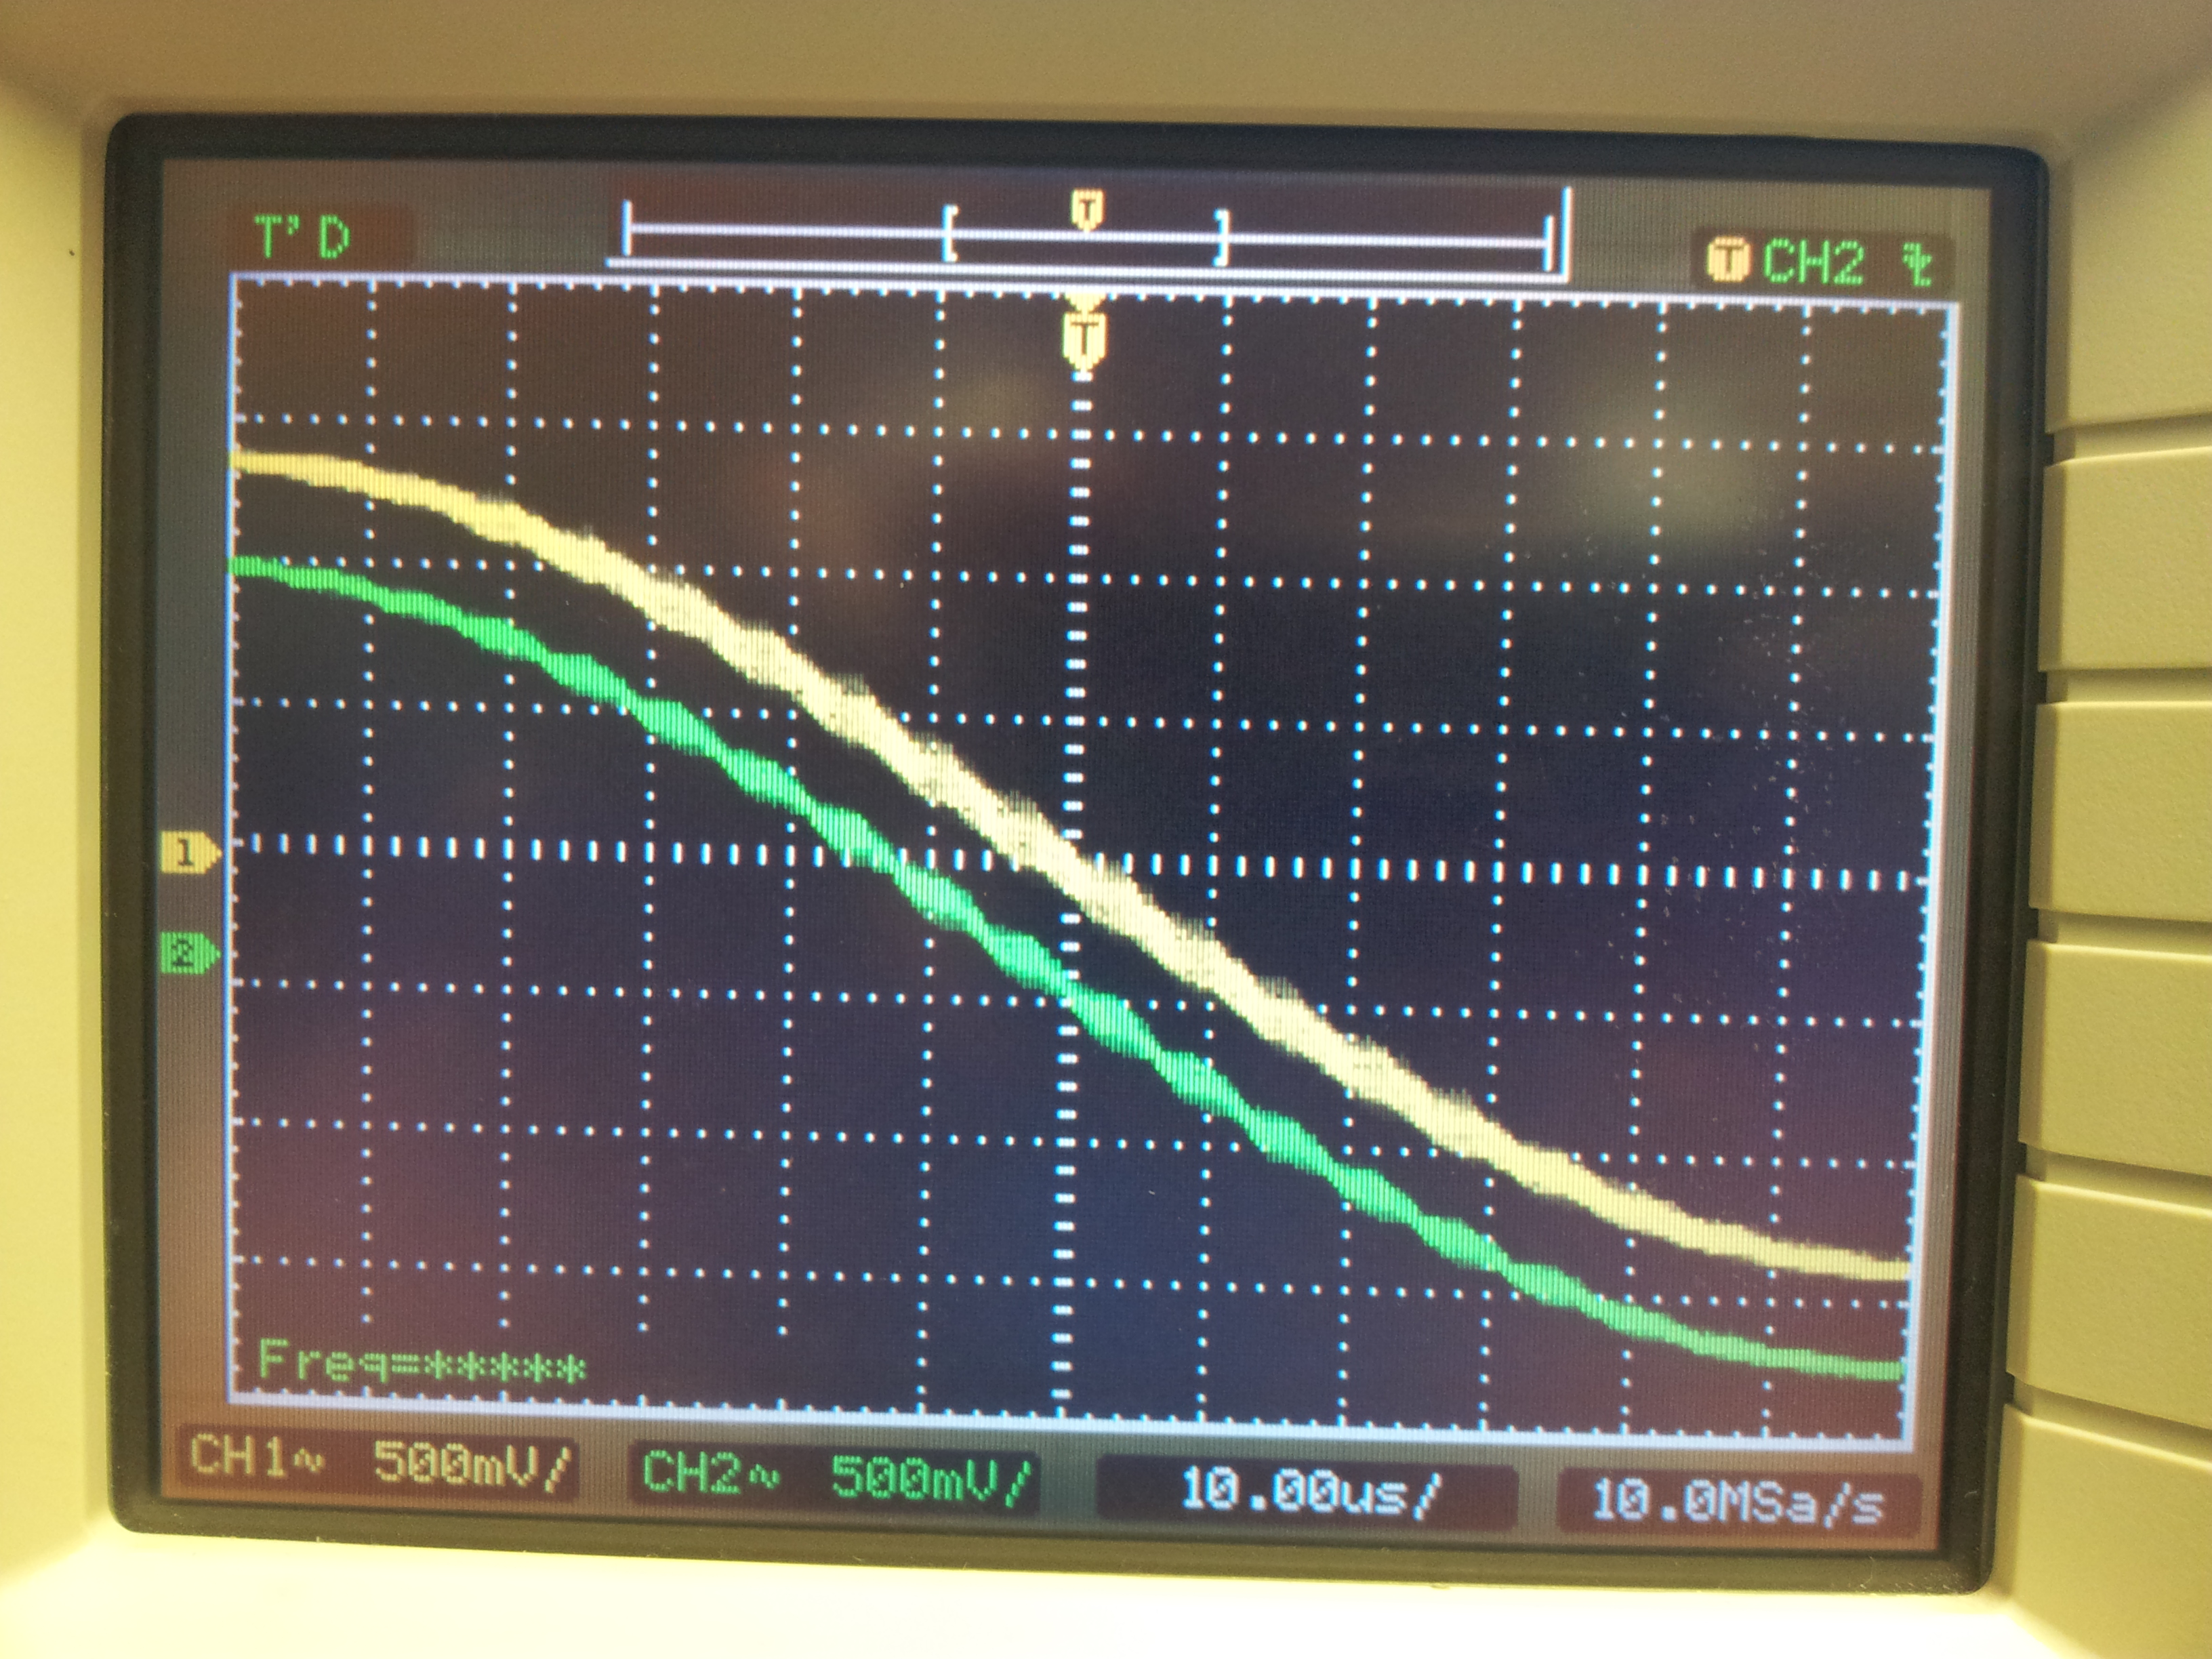
\includegraphics[width=0.5\textwidth]{./P1_interp}~\\
	\caption{Sinal sinusoide com interpolação(amarelo) e sem interpolação(verde).}
	\label{fig:interp}
\end{figure}

Nesta figura é possível observar os "degraus" mencionados anteriormente, tanto na onda interpolada como na onda não interpolada.
\paragraph{8.Comparação dos espectros com e sem interpolação} \hspace{0pt} \label{para:P1-8}

Não sendo possível estabelecer uma diferença entre os sinais com interpolação e sem interpolação foi necessário recorrer à observação dos espectros deles mesmos (Figuras \ref{fig:espect_s_interp} e \ref{fig:espect_c_interp}). Para estes sinais utilizou-se $\Delta_0=20479$ correspondente a $f_0=5kHz$.
\begin{figure}[H]
	\centering
	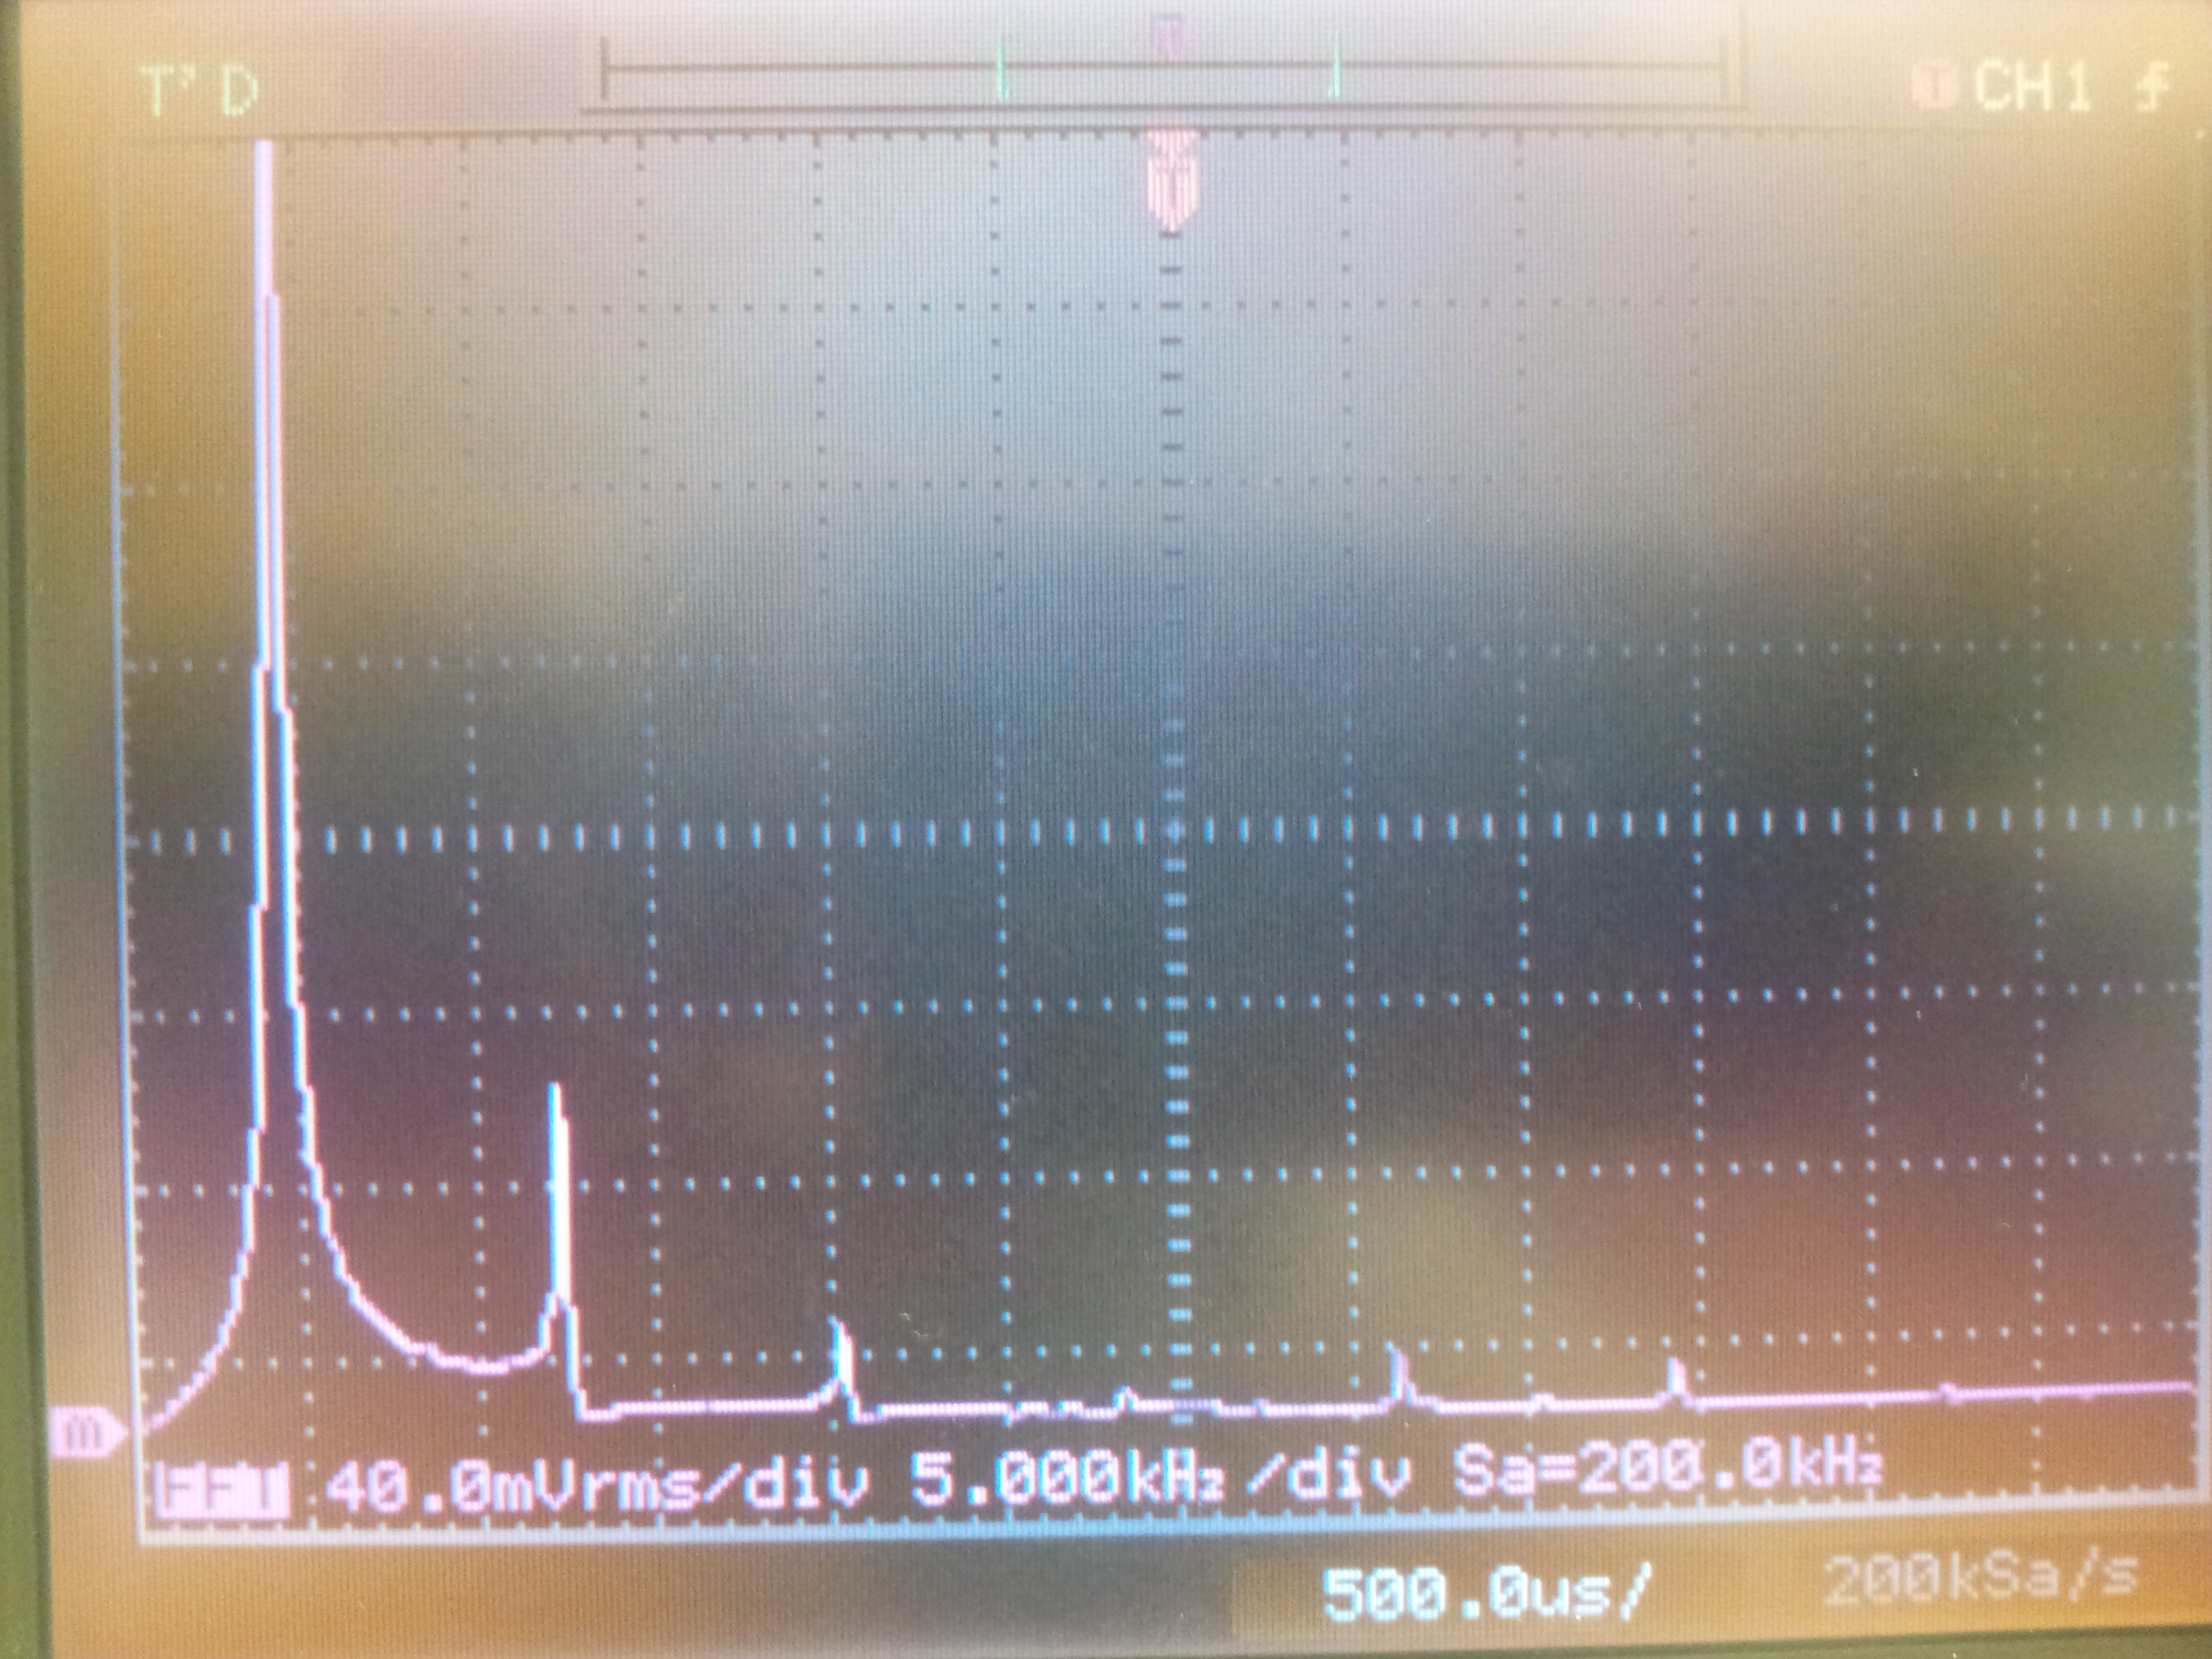
\includegraphics[width=0.5\textwidth]{./P1-8_espect_s_interp}~\\
	\caption{Espectro do sinal sinusoide sem interpolação.}
	\label{fig:espect_s_interp}
\end{figure}

\begin{figure}[H]
	\centering
	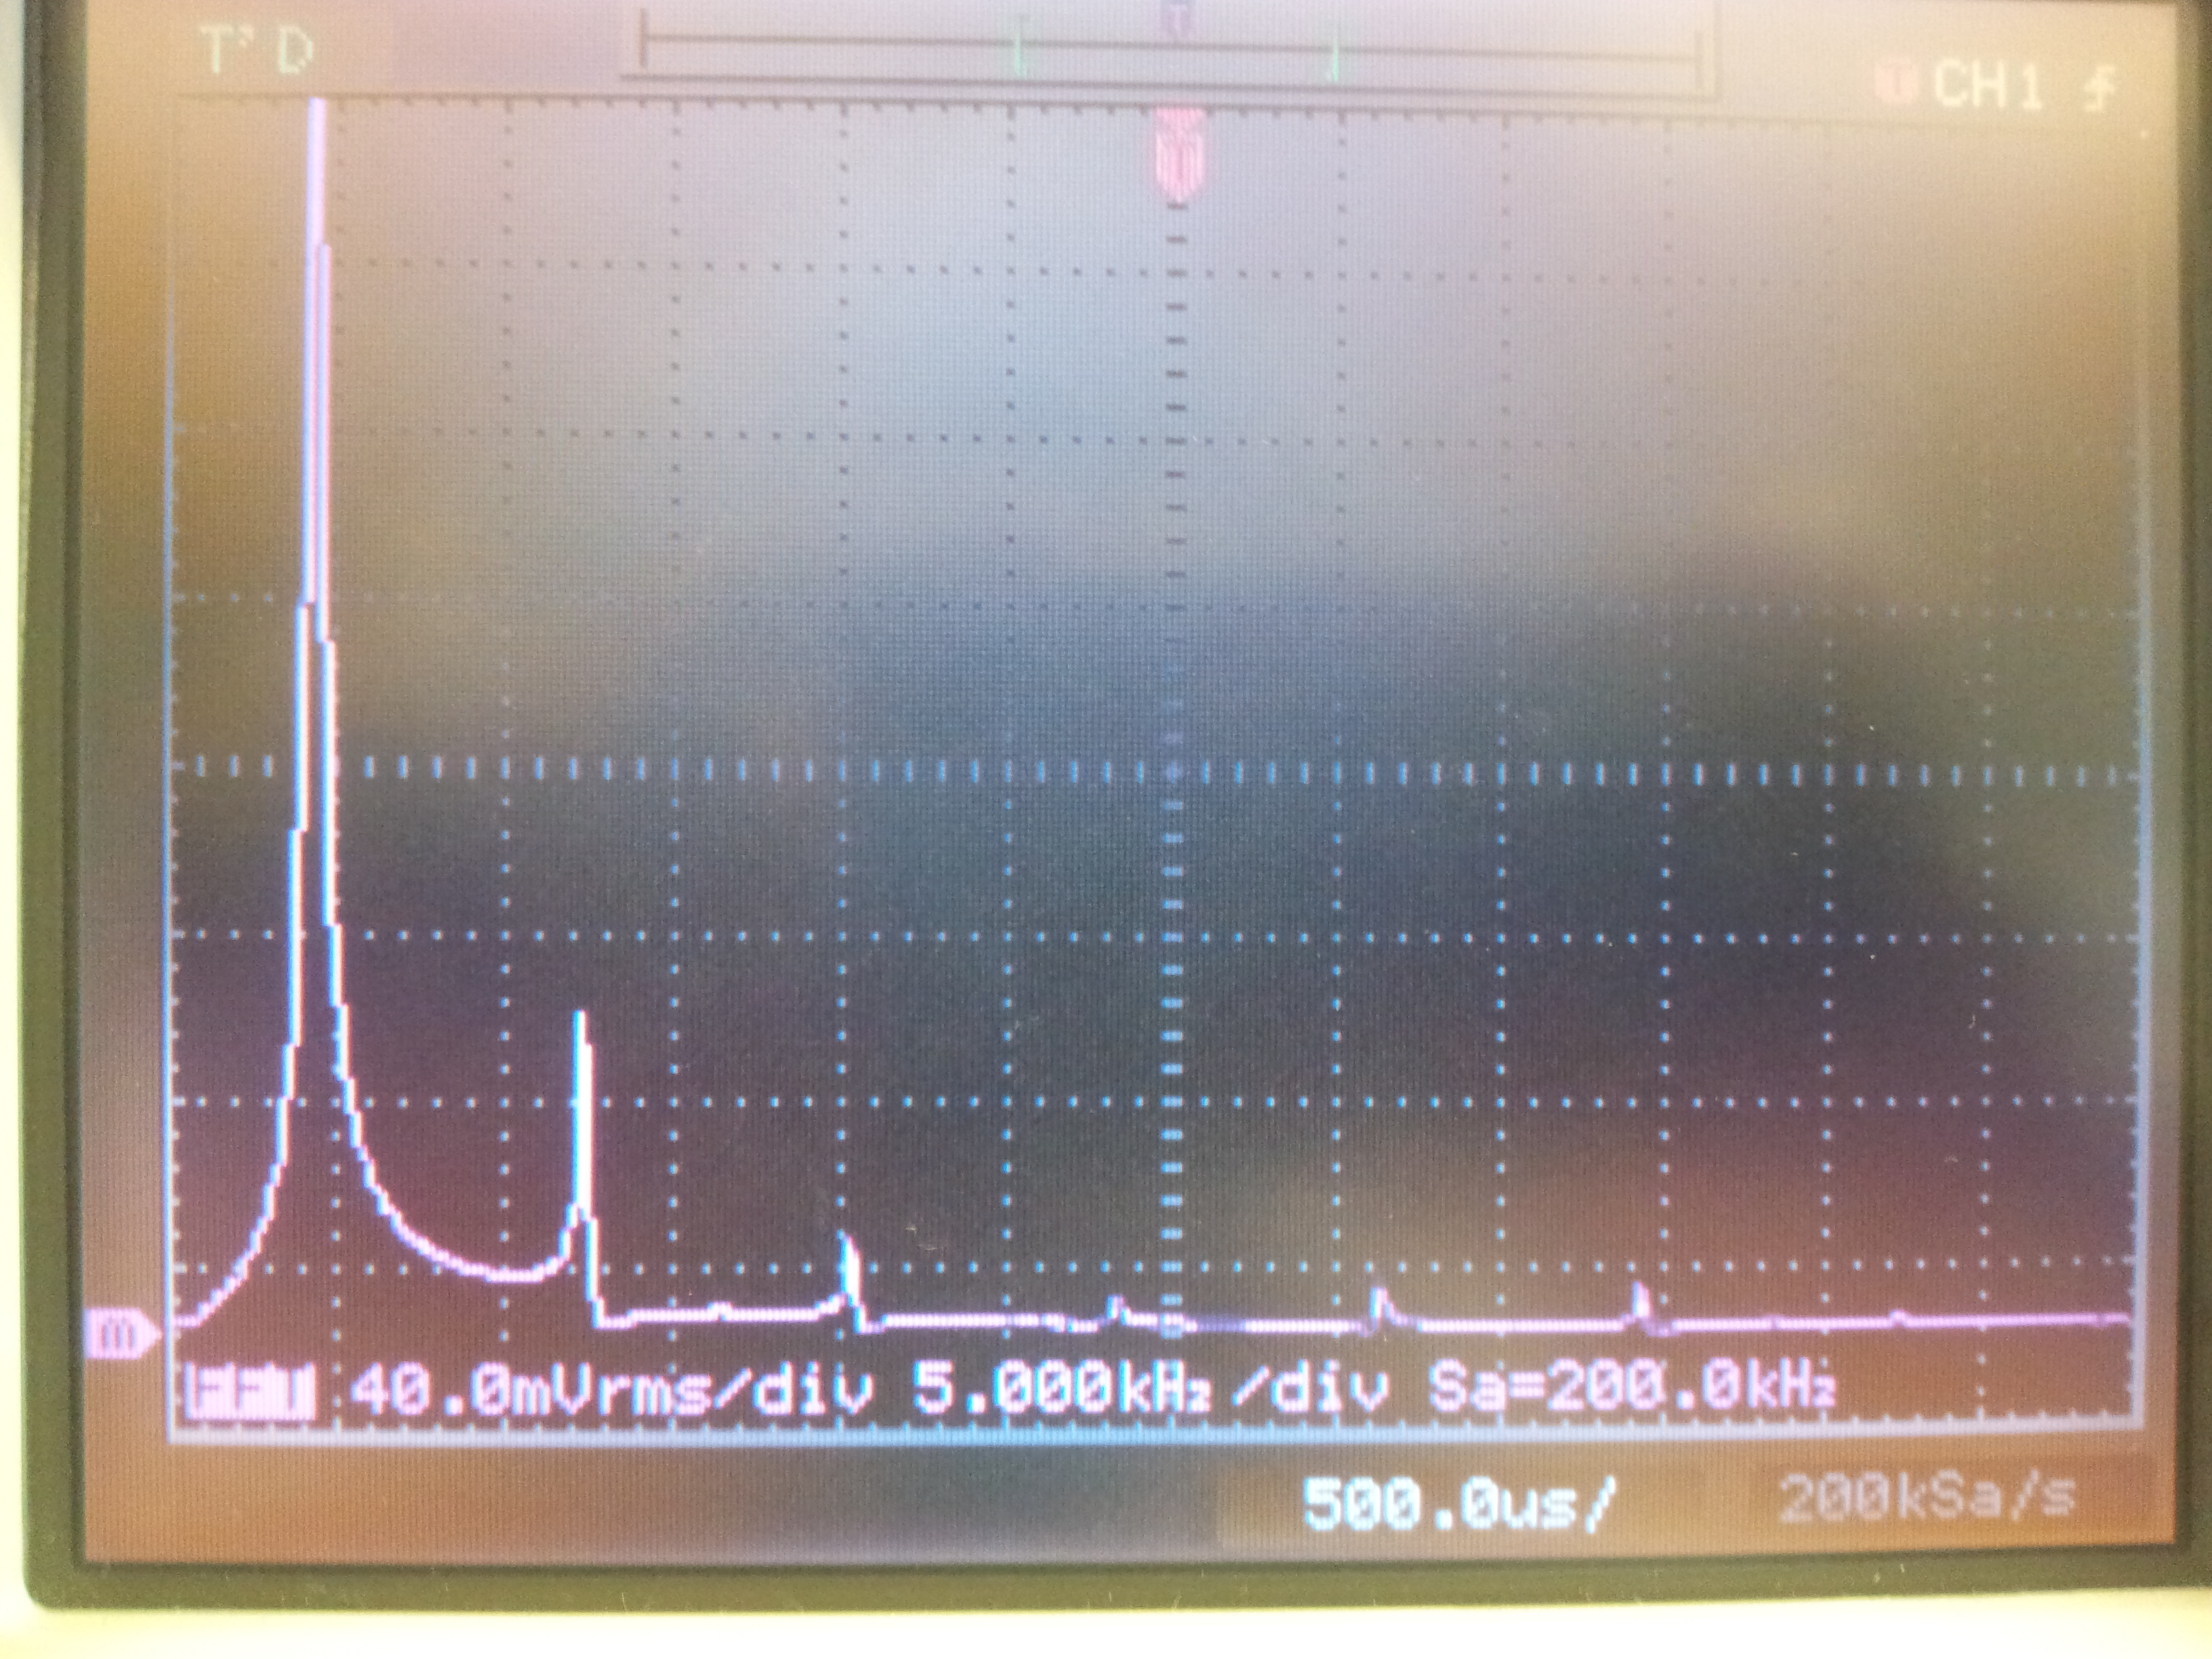
\includegraphics[width=0.5\textwidth]{./P1-8_espect_c_interp}~\\
	\caption{Espectro do sinal sinusoide com interpolação.}
	\label{fig:espect_c_interp}
\end{figure}

De novo não foi possível observar nas figuras diferenças visíveis entre os dois sinais, desta vez entre os seus espectros. Apresentam aparentemente a mesma amplitude para cada frequência entre eles mesmos.

A conclusão que se pode tirar com estas observações é que o método de interpolação, embora apresente uma melhor precisão dos valores, as melhorias não são observáveis pelos métodos e equipamentos usados.

\subsubsection{P2. Transmissor BPSK}
\label{p2}
%Introdução Teórica
O objectivo deste projeto é criar um transmissor BPSK com recurso a três elementos principais, uma fonte de bits, um codificador diferencial e mapeador, e um modulador.
Neste projeto foi utilizada uma frequência de amostragem $f_s=16$ kHz e uma frequência da portadora $f_0=4$ kHz.

\paragraph{1.Fonte de Bits} \hspace{0pt}
\label{para:P2-1}

Para ter uma fonte de bits no transmissor usa-se um "bit-rate clock" cuja função vai ser criar uma sequência de bits $ b_n $ com $f_b=1$ kbps. Isto significa que, considerando $f_s$, a cada 16 ciclos é gerado um novo bit, alternado em relação ao anterior. Assim, implementou-se um contador que é incrementado em cada ciclo  e que tem uma condição para verificar quando chegar ao valor 16. Ao entrar nessa condição é implementada a lógica para cálculo do novo bit da sequência e o contador é reiniciado.

Para calcular o novo bit basta negar o bit anteriormente obtido de modo a obter uma sequência de bits alternada, tendo sido concretizado este raciocínio com recurso uma simples XOR:
\begin{equation}
b_n=b_{n-1} \oplus 1
\end{equation}
Com esta operação, o bit resultante será sempre alternado em relação ao anterior.
Assim, obtém-se uma onda quadrada, observada no osciloscópio, que varia entre "0" e "1" e representa $ b_n $  com uma frequência de $500$ Hz(Figura \ref{bn_cn}). Esta frequência deve-se ao fato de se dividir  $f_b$ por dois pois cada meio ciclo da onda quadrada corresponde a um bit.  

\paragraph{2.Codificador Diferencial} \hspace{0pt} \label{para:P2-2}

Após obter a fonte de bits passou-se ao segundo elemento do transmissor: o codificador diferencial e mapeador. Começando pelo codificador diferencial, este serve para evitar ambiguidades na fase de maneira a poder sempre recuperar uma sequência de bits num canal que tenha sofrido uma variação na fase.
A codificação de $b_n$ resulta também de uma operação lógica XOR, como se pode observar: 
\begin{equation}
c_n=c_{n-1} \oplus b_n \hspace{3 mm} ,c_0=0
\end{equation}

Como um bit novo só é calculado quando o contador chega ao valor $16$, o mesmo também só é codificado nessa condição, ou seja, a cada 16 ciclos é codificado um bit. 

Tal como em $ b_n $ também $ c_n $ é representado por uma onda quadrada que varia entre "0" e "1" só que com o dobro do período, devido a só ter dois resultados para os quatro casos possíveis da XOR que realiza a codificação(Figura \ref{bn_cn}).
\begin{figure}[H]
	\centering
	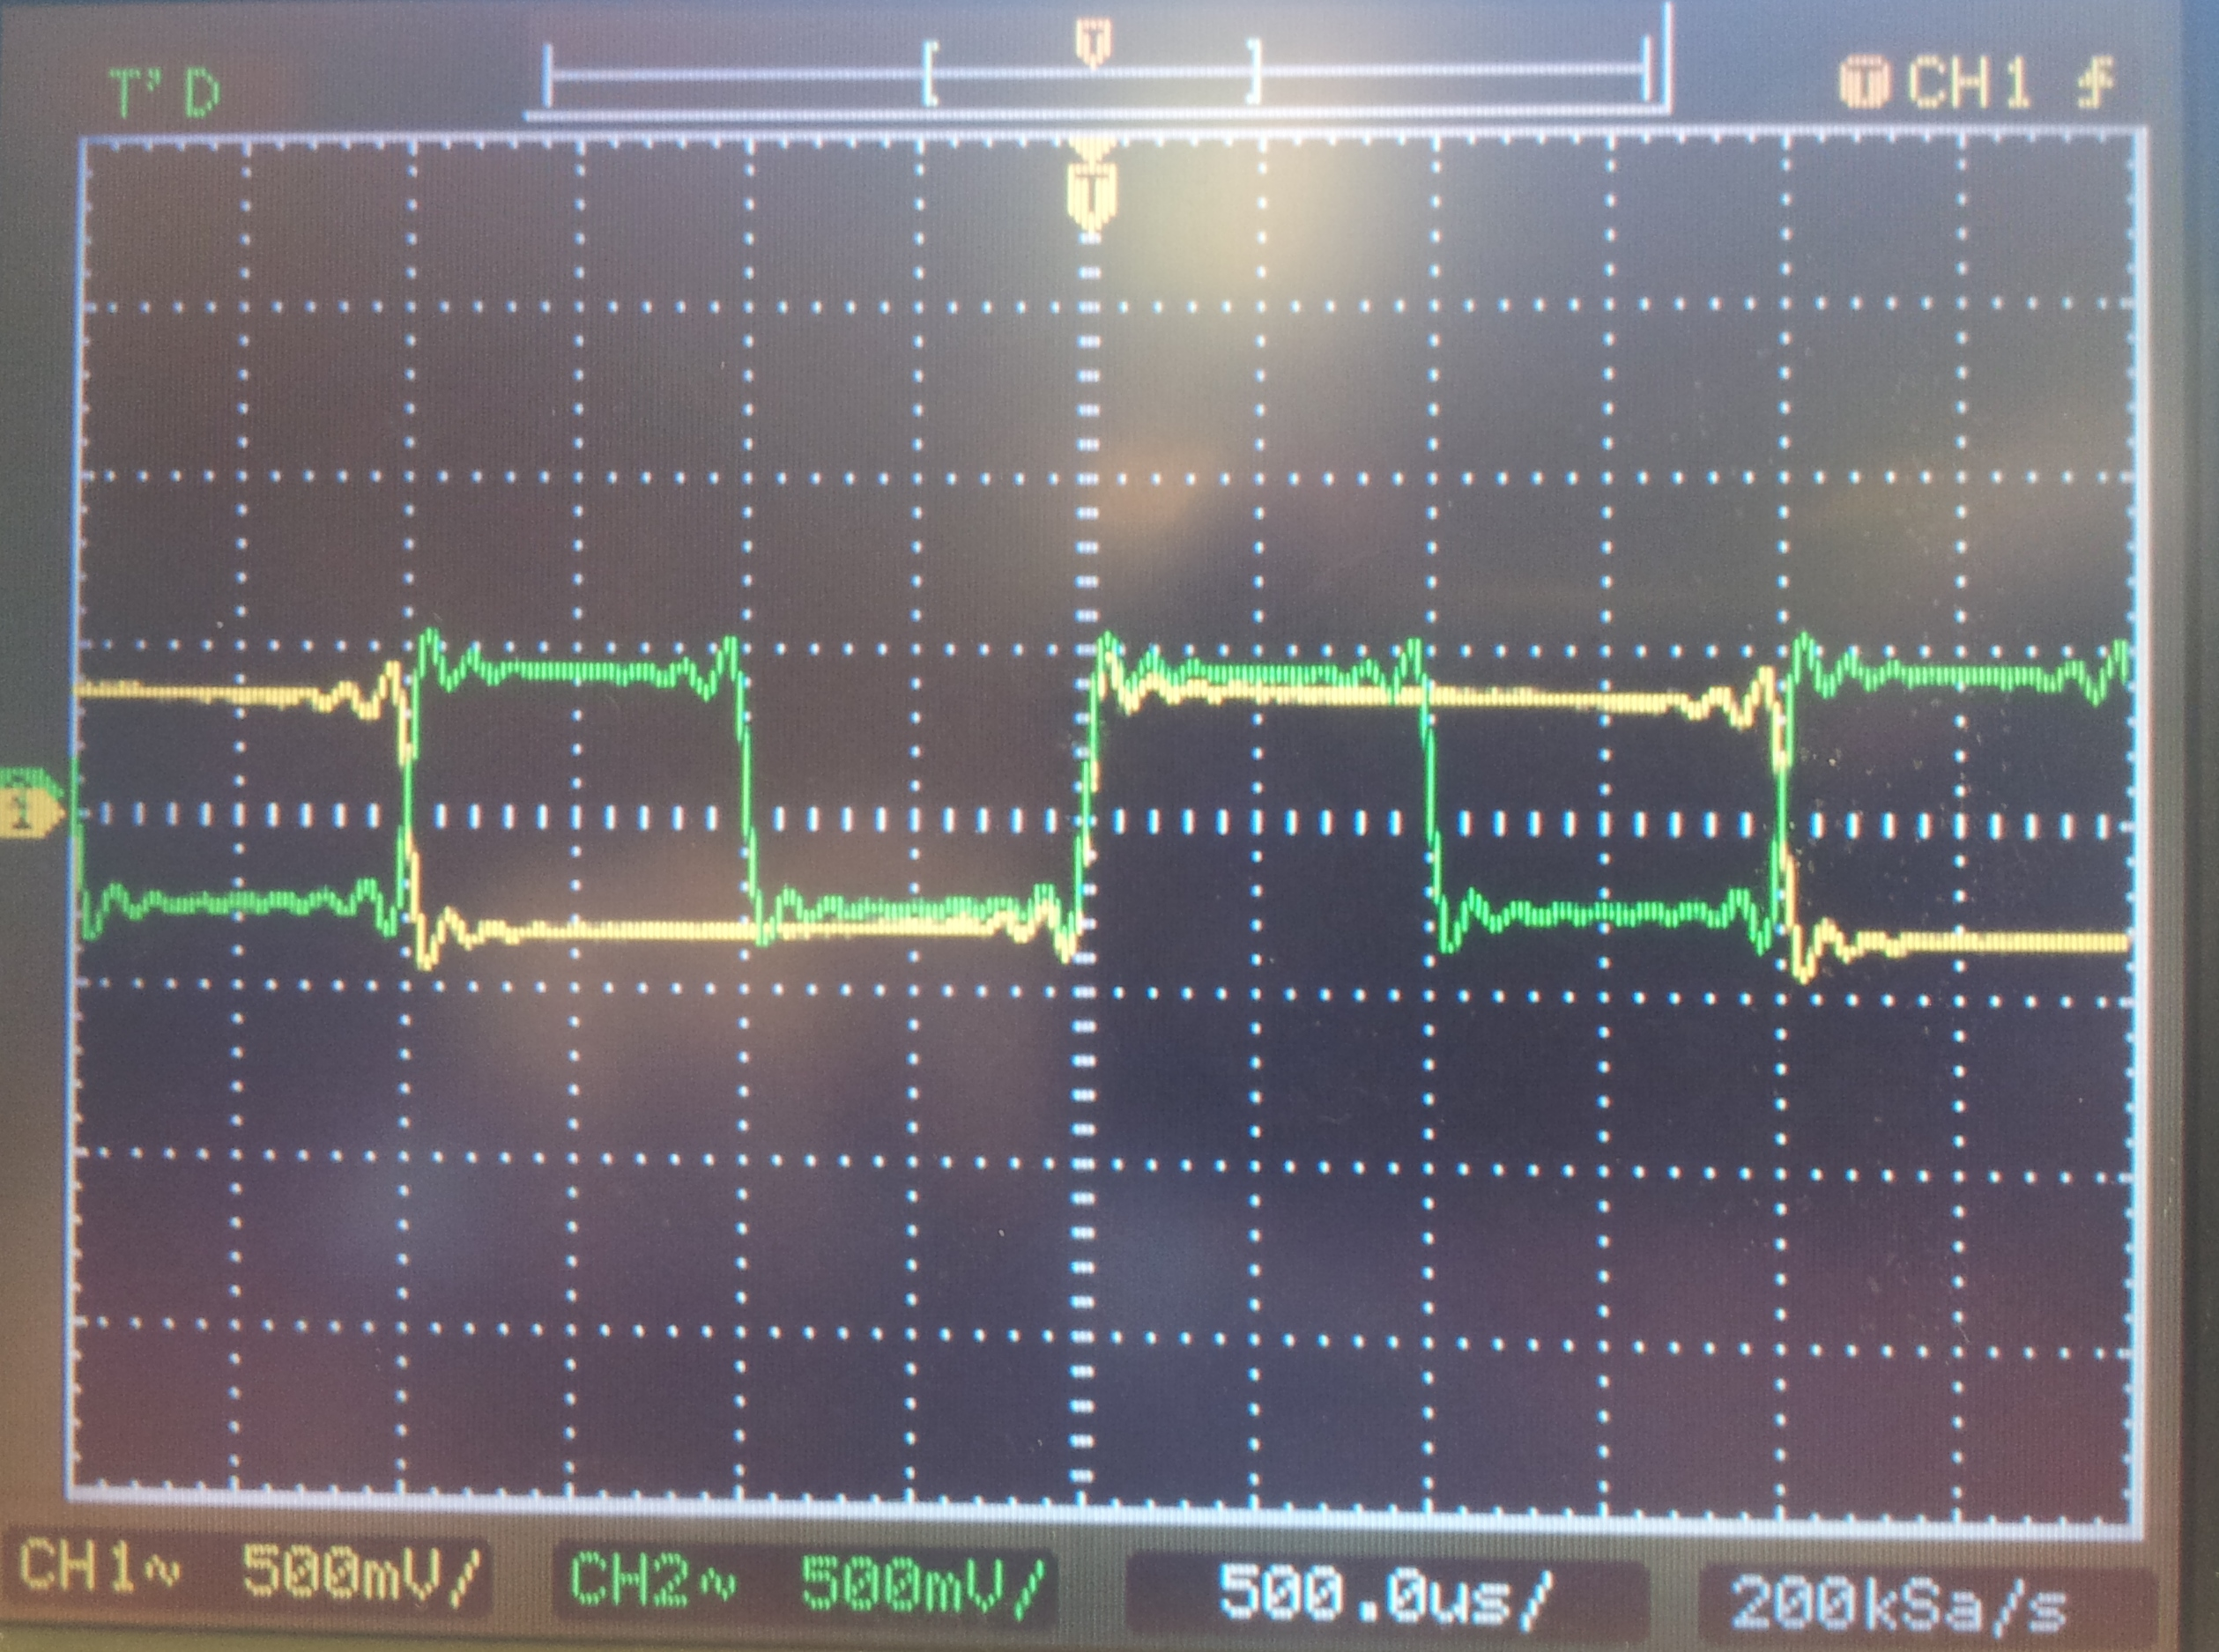
\includegraphics[width=0.5\textwidth]{./bn_cn}~\\
	\caption{$ b_n $(verde) e $ c_n $(amarelo)}
	\label{bn_cn}
\end{figure}

\paragraph{3.Mapeador} \hspace{0pt}
\label{para:P2-3}

Depois de obter $ c_n $ passa-se ao mapeamento do mesmo. O mapeamento baseia-se em duas condições:
\begin{equation}
	c_n= '1' \rightarrow d_n =+1 \hspace{5 mm} c_n='0' \rightarrow d_n=-1
\end{equation}

Esta lógica podia ser facilmente implementada com recurso a duas condições "if", mas optou-se por evitar essa lógica para tornar o programa mais eficiente.
Assim recorreu-se a um \textit{shift} e a uma subtração. Atenção que esta não é a maneira mais eficiente pois a subtração faz com que o programa tenha de passar pela ALU.
Pode-se observar então o mapeamento efetuado através da seguinte expressão:
\begin{equation}
d_n=32767*((c_n << 1)-1)
\end{equation}

Antes de mais, o ganho que está a ser multiplicado é utilizado para converter o resultado em Q15, como já foi feito anteriormente. Considerando a expressão sem esse ganho, vê-se que para $ c_n=0 $, como o \textit{shift} não influencia o resultado, o mesmo só depende da subtração e é sempre o pretendido, $d_n=-1$. Se $c_n=1$, o \textit{shift} duplica  esse valor, e depois ao subtrair obtém-se $d_n=1$.

Tal como em $b_n$ e $c_n$ esta operação só é executada a cada 16 ciclos pois depende diretamente de $c_n$ e só se mapeia um novo bit depois de ele ser codificado. Concluído o mapeamento obtém-se mais uma vez uma onda quadrada mas desta vez varia entre "-1" e "1" (figura \ref{cn_dn}).
\begin{figure}[H]
	\centering
	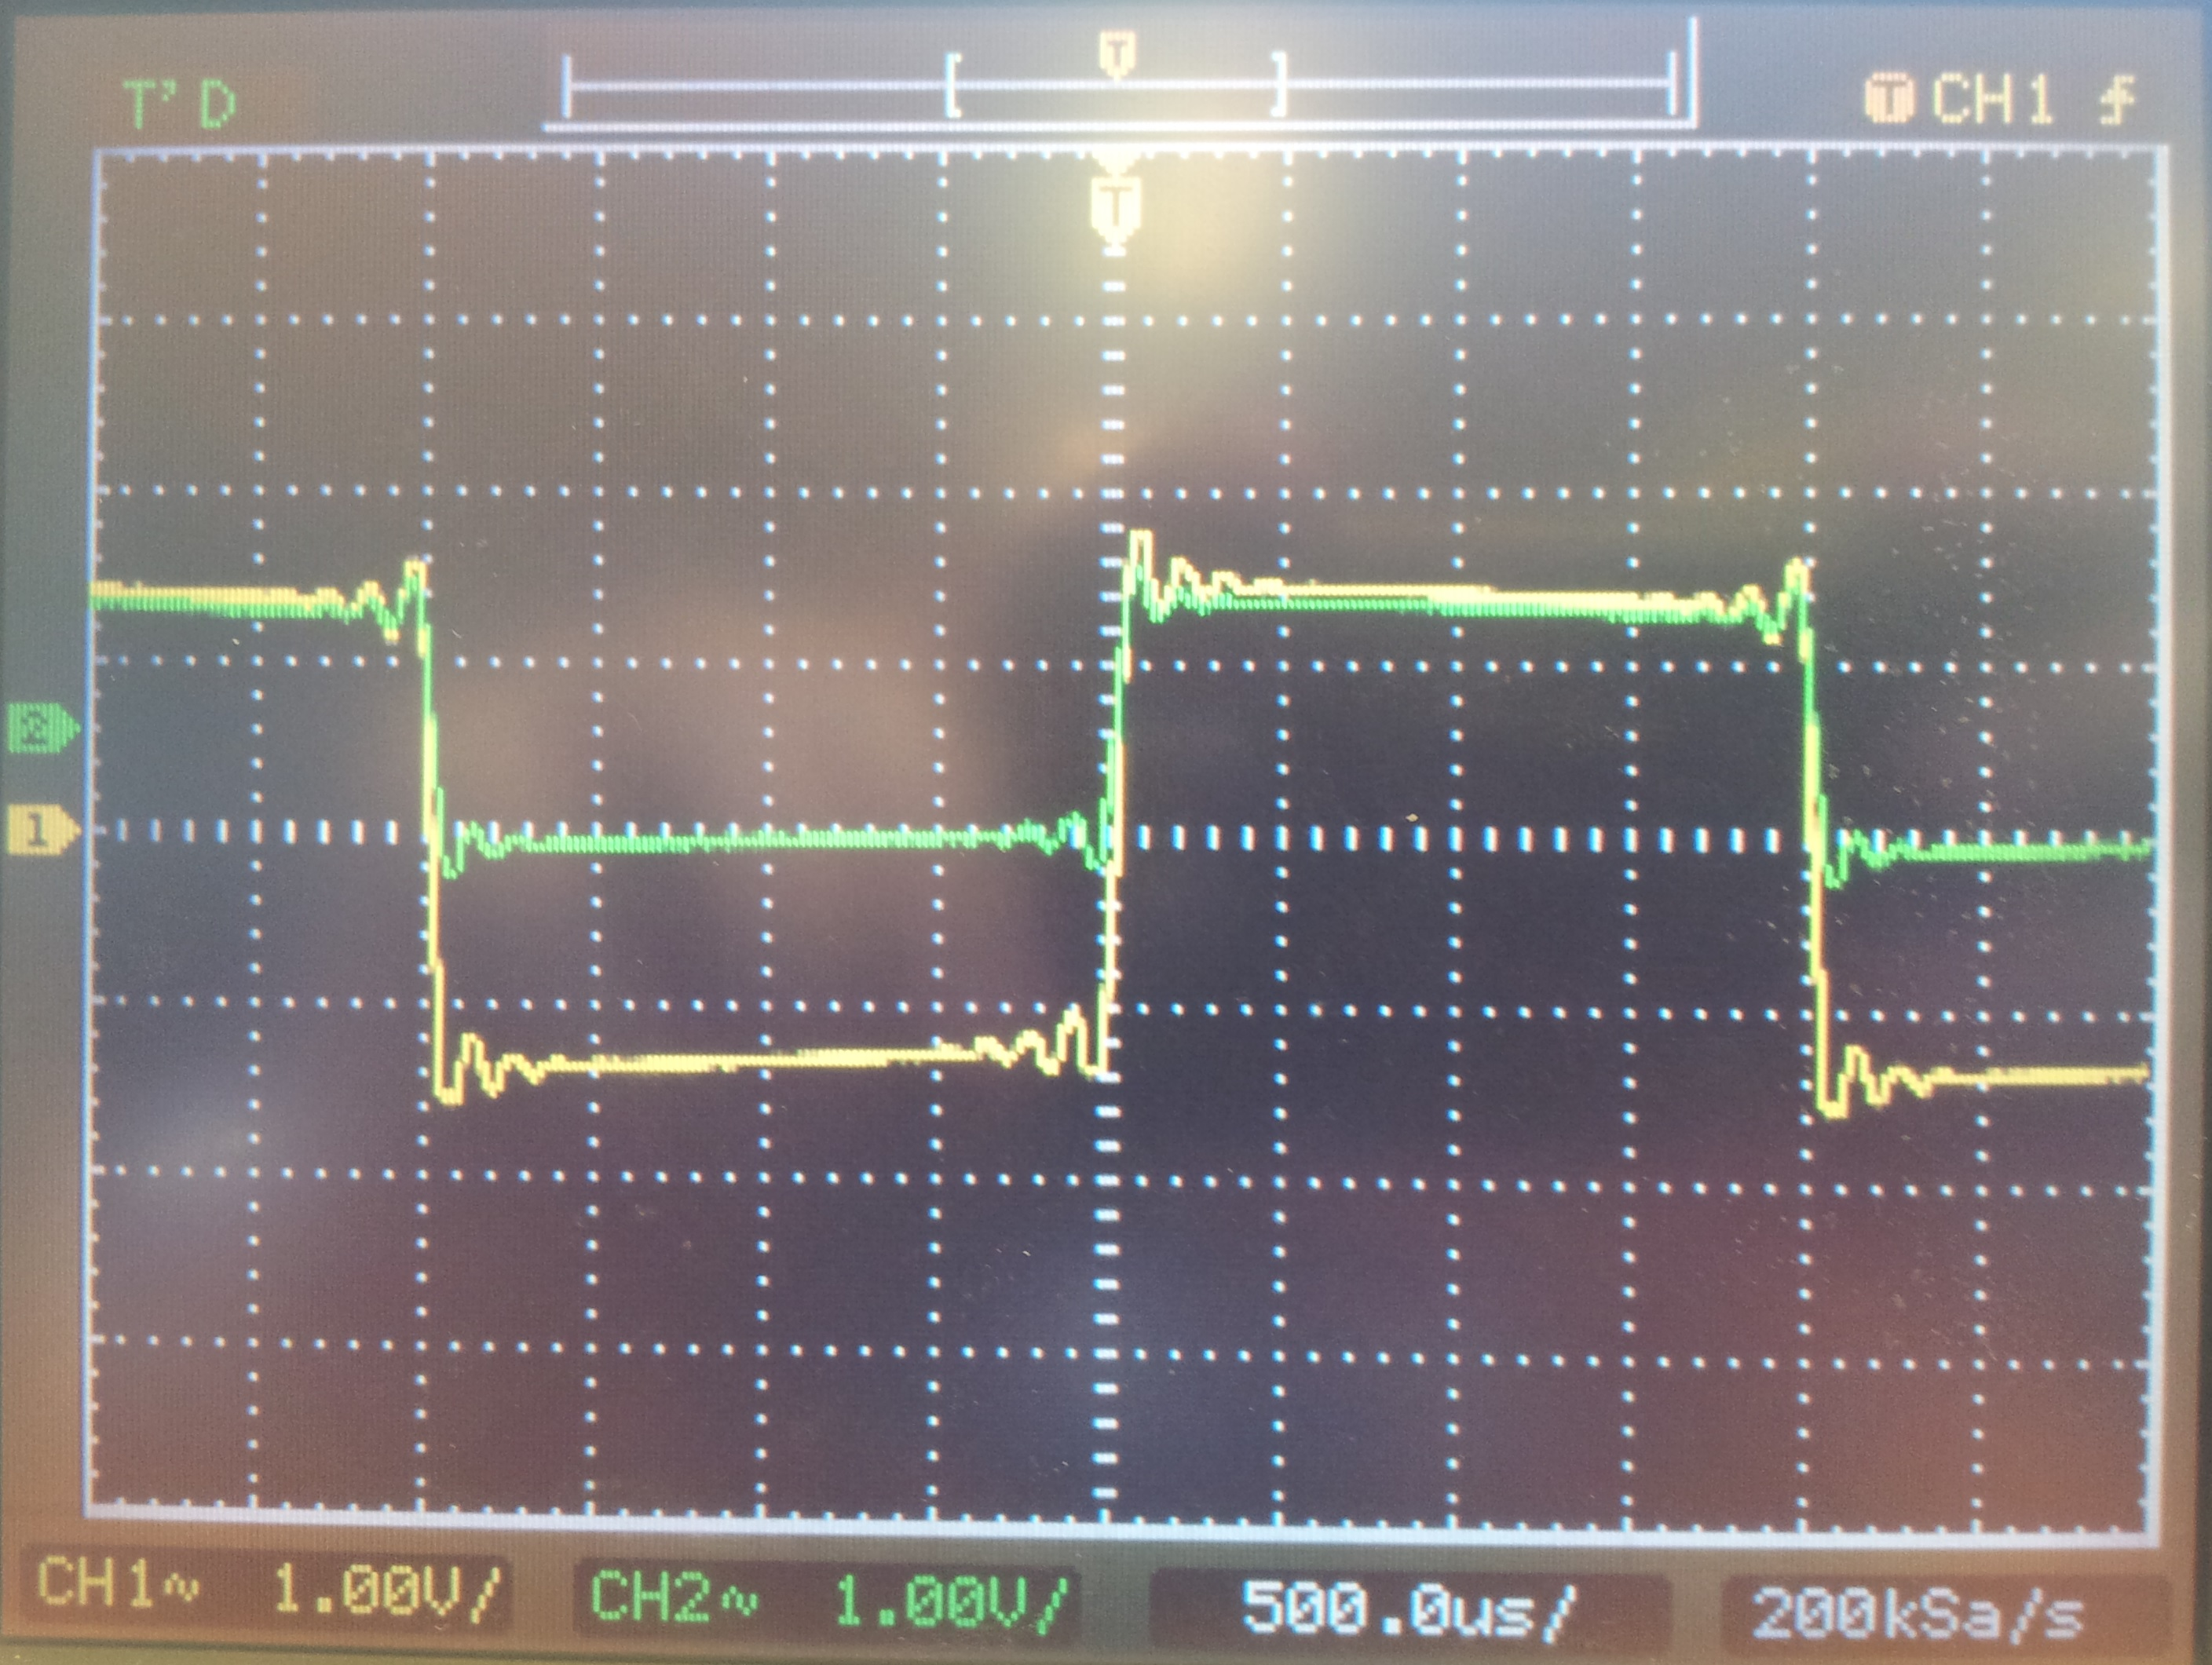
\includegraphics[width=0.5\textwidth]{./cn_dn}~\\
	\caption{Formas de onda de $d_n$ (amarelo) e $c_n$ (verde).}
	\label{cn_dn}
\end{figure}

\paragraph{4.Implementação do Modulador} \hspace{0pt}
\label{para:P2-4}

Falta agora gerar a onda portadora a modular. Esta foi implementada de forma mais simples face ao projeto anterior uma vez que a frequência é constante (4 kHz) e este valor consiste numa fração inteira da frequência de amostragem ($16 kHz$).
Em primeiro lugar criou-se uma tabela com quatro valores dum período da sinusóide, sendo esta:
\begin{table}[H]
	\centering
	\caption{Amostras da onda portadora}
	\label{tab:amostras}
	\begin{tabular}[c]{|l||c|}
		\hline \textbf{contador} & \textbf{seno}\\ 
		\hline $ 0 $ & $ 0 $\\ 
		\hline $ 1 $ & $ 32767 $  \\ 
		\hline $ 2 $ & $ 0 $ \\ 
		\hline $ 3 $ & $ -32767 $ \\
		\hline
	\end{tabular}
\end{table}

Escolheram-se estes valores uma vez que o período de amostragem coincide com os instantes de máximo, mínimo e \textit{zero-crossing} da portadora. Para gerar a portadora (Figura \ref{port_mod}) recorreu-se a um contador que, em cada interrupção (ocorrendo em cada instante de amostragem, como explicado no enunciado), aponta para cada entrada da tabela e põe a amostra numa variável que, após se incrementar o contador, irá ser multiplicada por $d_n$. Esta tabela não gera uma onda triangular pois das harmónicas destas, abaixo da frequência de amostragem ( $f_0$=4kHz e 3$f_0$=12kHz) apenas a primeira harmónica se encontra na banda de passagem do filtro de reconstrução do DAC, que terá frequência de corte Fs/2.

A onda modulada é então representada pela seguinte expressão:
\begin{equation}
	s_n= d_n \sin(2 \pi f_0T_sn) 
\end{equation}
Neste caso os valores do seno são os valores das amostras discutidas anteriormente.
\vspace{2 mm}
                                              
\paragraph{5.Teste do Modulador BPSK} \hspace{0pt}
\label{para:P2-5}

Após implementar o modulador, tem-se o transmissor BPSK completo e para testá-lo, pôs-se nos dois canais do osciloscópio a onda portadora e a onda modulada (Figura \ref{port_mod}).
\begin{figure}[H]
	\centering
	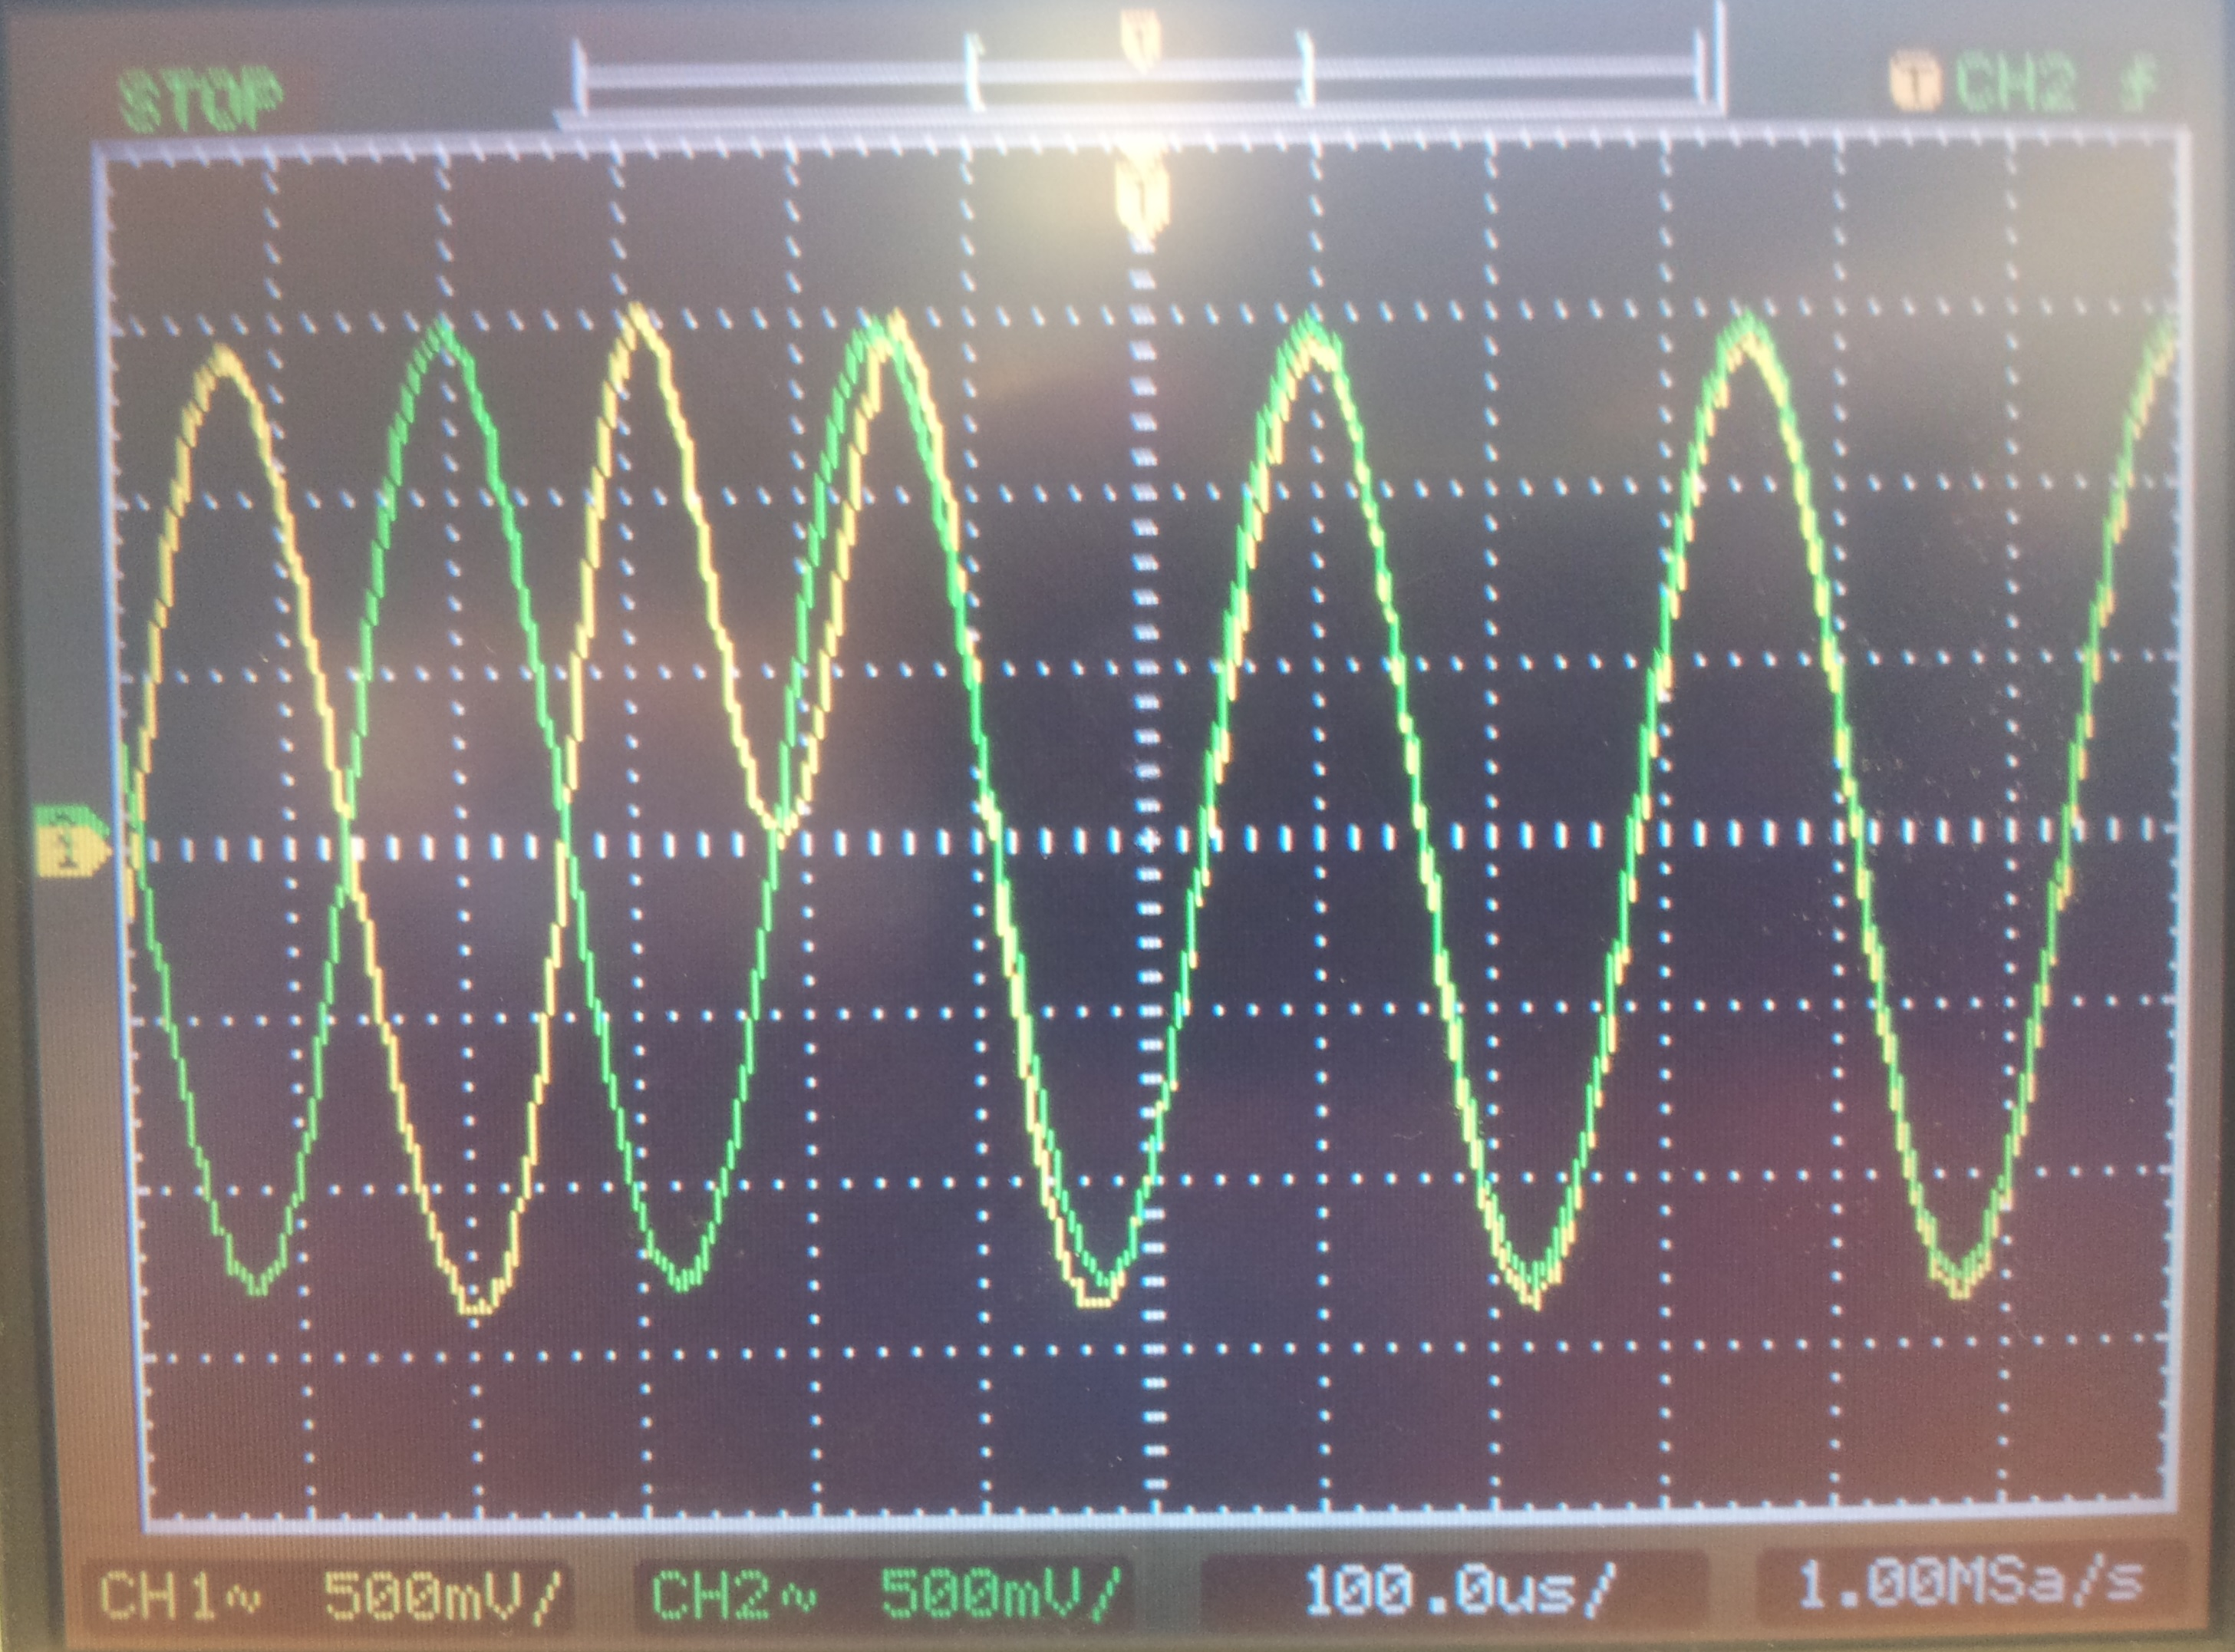
\includegraphics[width=0.5\textwidth]{./port_mod}~\\
	\caption{Onda portadora (verde) e onda modulada (amarelo)}
	\label{port_mod}
\end{figure}
 \vspace{2 mm}
 
 Como se pode observar pela imagem e considerando a expressão (8), a onda portadora começa em oposição de fase com a onda modulada. Isto ocorre quando $d_n=-1$, o que significa que quando $d_n=1$ a onda modulada é igual à portadora. É possível observar quando $d_n$ muda de valor pois é exatamente quando a onda modulada inverte a sua fase (Figura \ref{dn_mod}). 
 \begin{figure}[h]
 	\centering
 	\subfloat[]{\includegraphics[width=0.4\textwidth]{./dn_mod2}}
 	\hspace{6 mm}
 	\subfloat[]{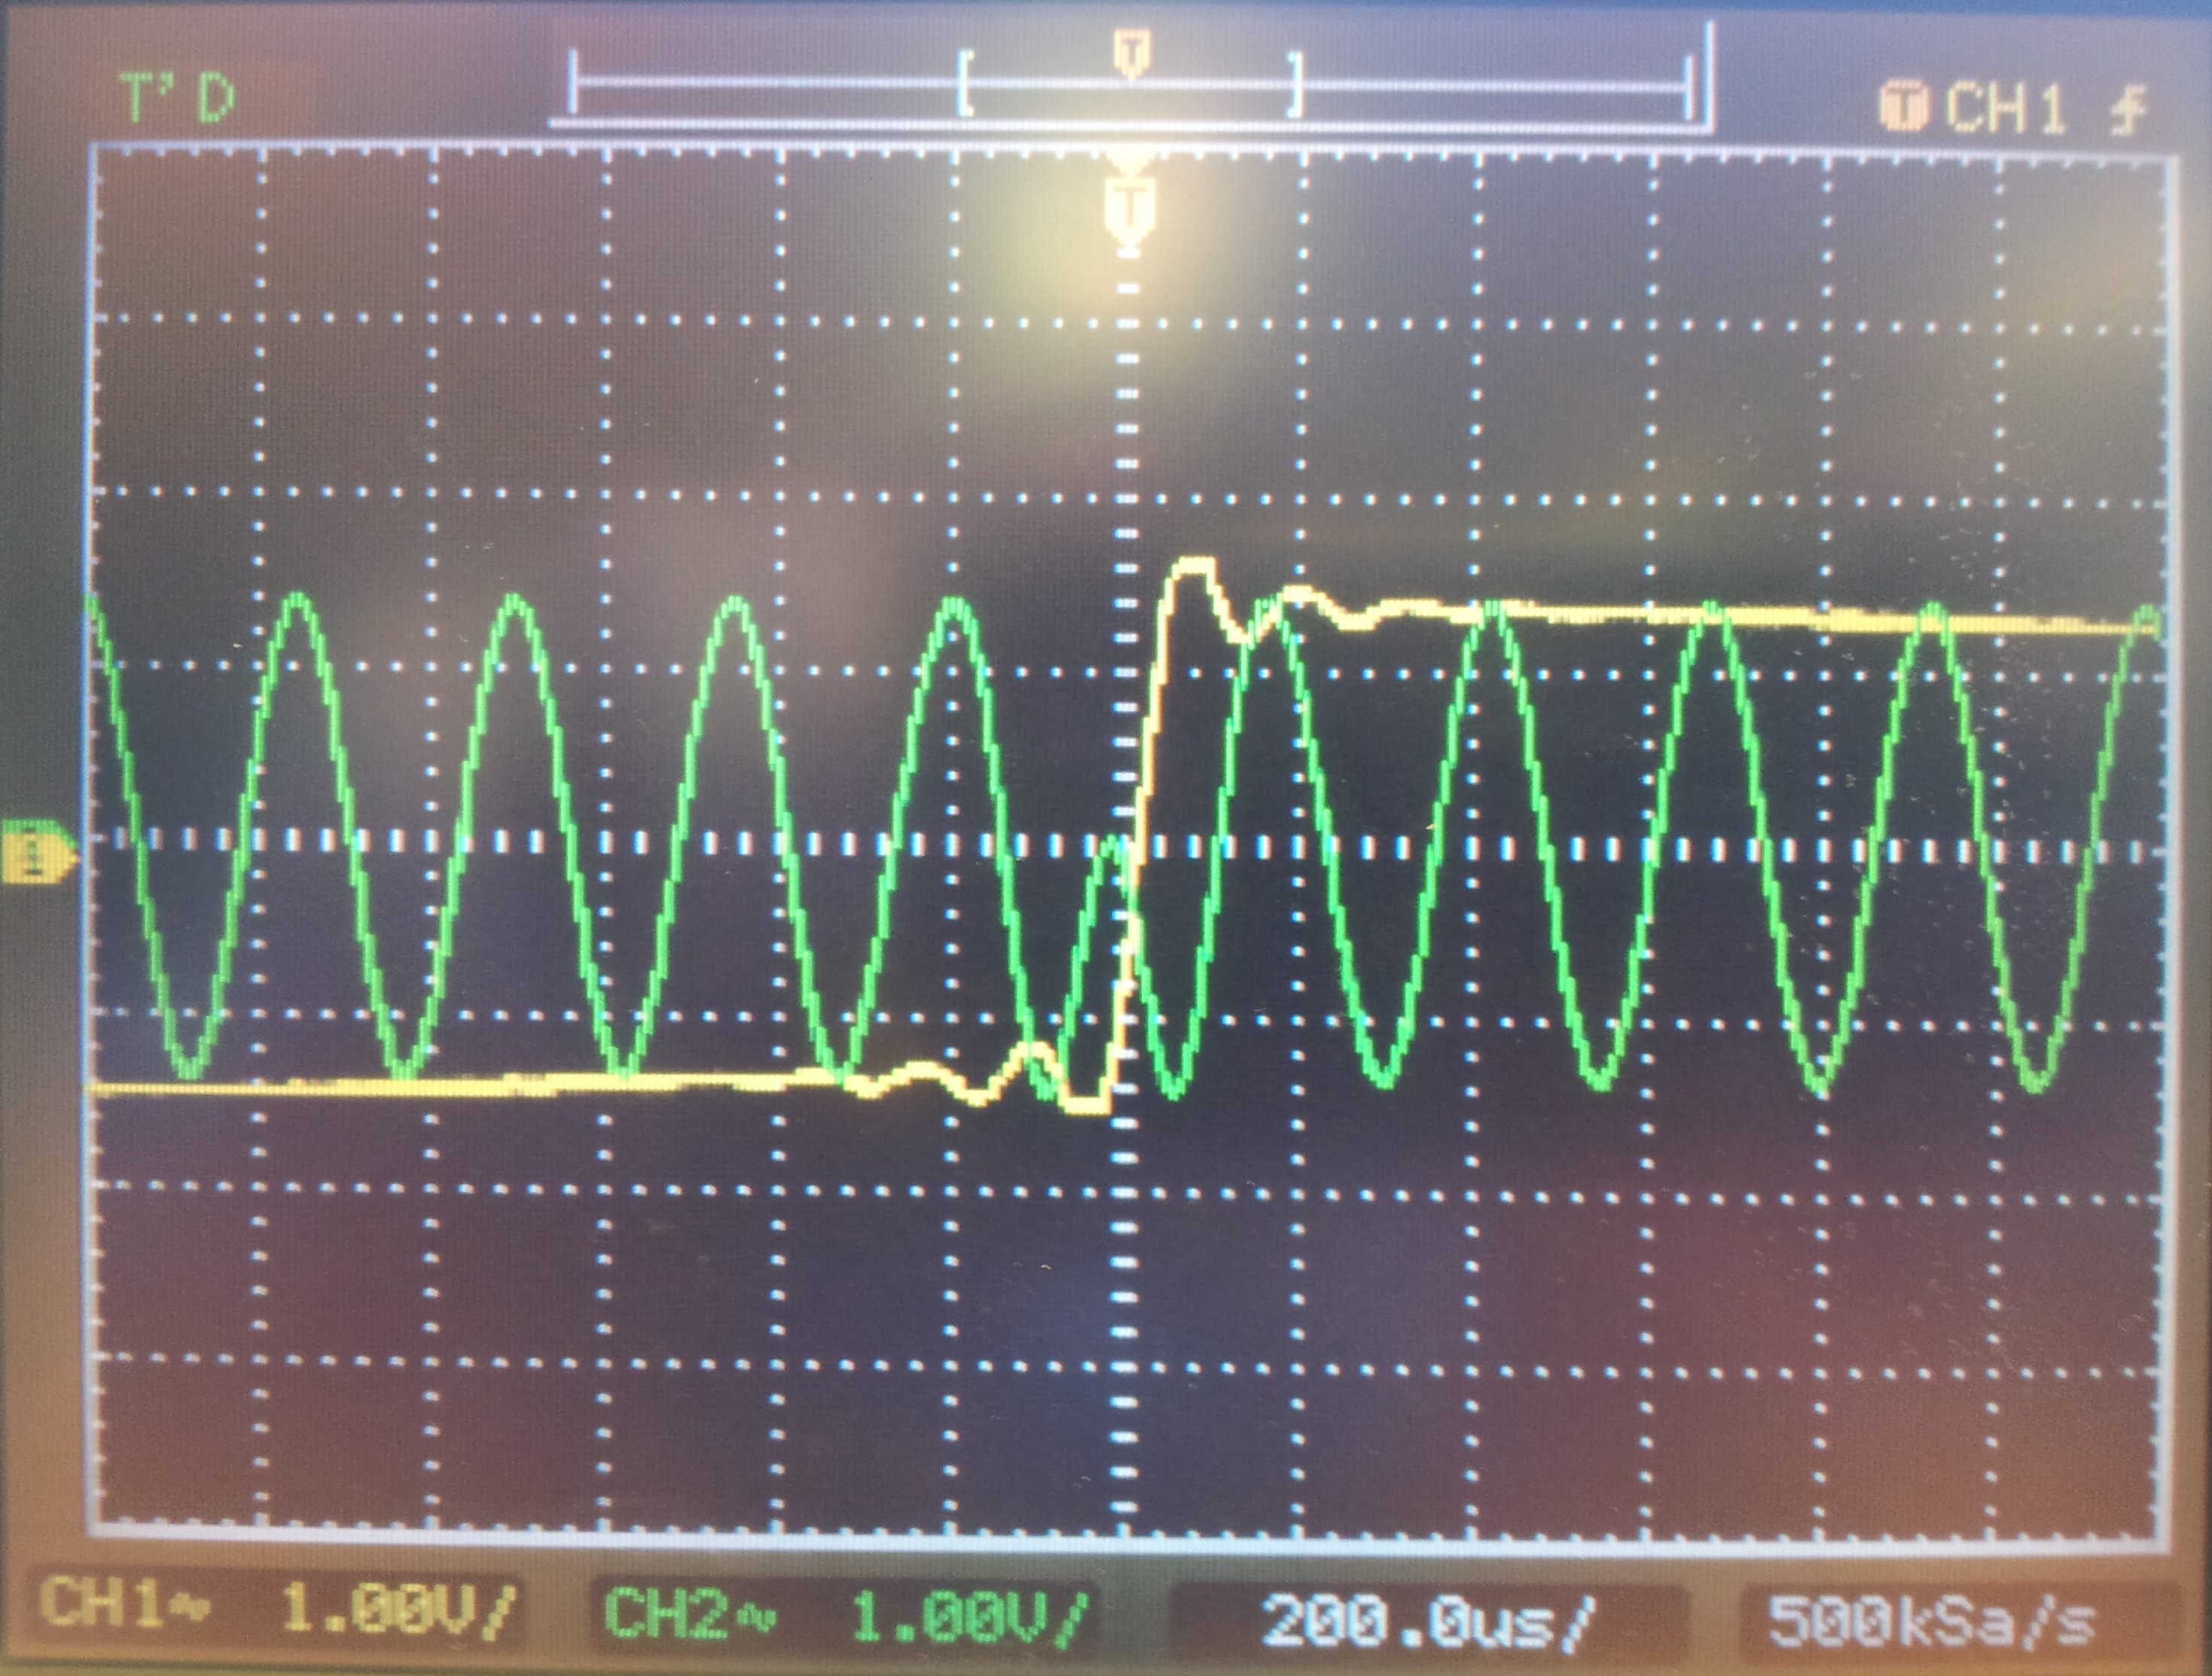
\includegraphics[width=0.4\textwidth]{./dn_mod}}
 	\caption{Formas de onda de $d_n$ (amarelo) e $s_n$ (verde), zoom em (b)}
 	\label{dn_mod}
 \end{figure}
 
 Este fenómeno acontece a cada 8 ciclos pois, como já foi explicado anteriormente, a frequência da onda correspondente à fonte de bits é o bit-rate dividido por dois e uma vez que a codificação divide esta frequência por dois, ou seja, a frequência de $d_n$ é 250 Hz e por isso cabem oito ciclos da portadora num meio ciclo de $d_n$.
 \vspace{2 mm}

\paragraph{6.Espectro do Sinal Modulado} \hspace{0pt}
\label{para:P2-6}

Para compreender melhor o sinal modulado, observou-se o espetro do mesmo (Figura \ref{espetro}).
\begin{figure}[H]
	\centering
	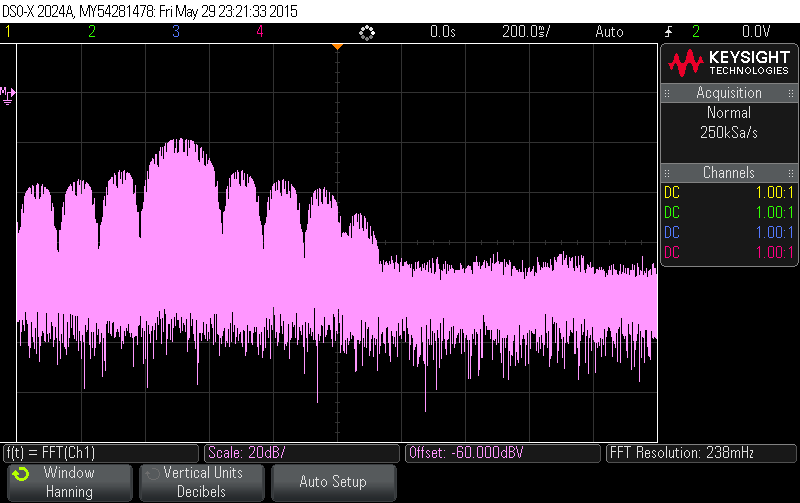
\includegraphics[width=0.5\textwidth]{./spectrum_sn_0-16k}~\\
	\caption{Espectro do sinal $s_n$.}
	\label{espetrosn}
\end{figure}

A onda modulada no tempo consiste na multiplicação de uma onda quadrada com uma onda sinusoidal, na frequência isto consiste na convolução do espetro da primeira, um $sinc$, com o espetro da segunda, um impulso em $f_0$. Isto resultaria numa translação do espetro da onda quadrada, ficando centrado na frequência da onda sinusoidal.

Na imagem acima vê-se o espectro de $d_n$ centrado em 4kHz como esperado. O espetro tem o \textit{SPAN} [0-16KHz] e apresenta a forma descrita acima, exceto a falta de réplica a 16kHz, contudo isso é explicado pelo filtro anti-aliasing do analisador de espetros.

consiste na convolução do espetro da primeira (impulsos nos múltiplos ímpares da frequência fundamental) com o espetro da segunda (um impulso à frequência $f_0$). Isto resultaria numa translação do espetro da onda quadrada, ficando centrado na frequência da onda sinusoidal.

Na imagem acima vê-se o espectro de $d_n$ centrado em 4kHz como esperado. Como se pode observar, as harmónicas de maior amplitude estão espaçadas 250 Hz em relação a $f_0$ indicando que a frequência fundamental da onda quadrada é 250 Hz, como esperado.

\subsubsection{Receptor \textit{Costas Loop}}
Com o transmissor de BPSK e NCO completos, resta desenvolver o recetor com a capacidade de desmodular o sinal BPSK. Para tal, em vez de optarmos por um circuito do tipo phase-locked loop (PLL) e detetor coerente, desenvolveu-se um desmodulador com o circuito \textit{Costas Loop}. Este é baseado em PLL, contudo tem o dobro da sensibilidade pois tem um detetor de fase para a componente em fase e para a componente em quadratura sendo estes sinais multiplicados , na malha de retroação, resultando num sinal com o dobro do erro para usar no NCO. Tem a vantagem de desmodular sinais com \textit{Doppler shift}. Para este recetor ser utilizado com sucesso, em primeiro lugar o transmissor e o NCO têm que sofrer algumas alterações.

\paragraph{1.Introdução do \textit{Scrambler}:} \hspace{0pt}
\label{para:P3-1}

\todo{guilherme}

Para um bom funcionamento do Costas Loop é necessário um \textit{scrambler}. O \textit{Scrambler} tem como função não permitir que á entrada se verifique uma longa sequência de '1's ou de '0's, pois estas podem causar uma dessincronização momentânea do sistema. Outra causa para dessincronizações momentâneas do sistema é o aparecimento de sequências periódicas à entrada. A utilização de um \textit{Scrambler} é o  método utilizado para diminuir o riscos de dessincronização momentânea.
\begin{figure}[H]
	\centering
	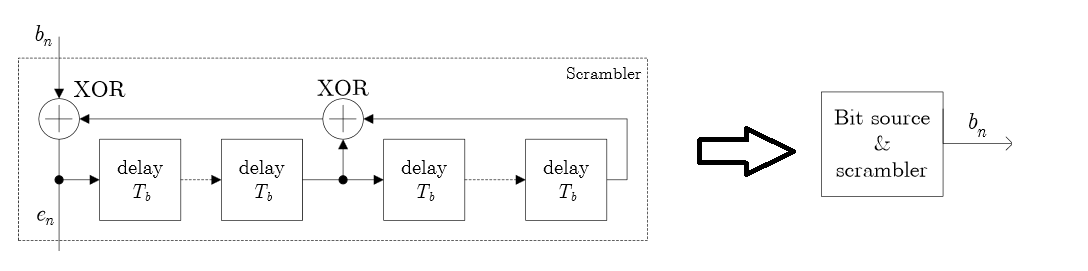
\includegraphics[width=0.8\textwidth]{./Scrambler}~\\
	\caption{Modelo do \textit{Scrambler} a contruir.}
	\label{fig:scrambler}
\end{figure}

A Figura \ref{fig:scrambler} representa o \textit{scrambler} a implementar, nas Equações \ref{eq:scrambler_1}, \ref{eq:scrambler_2} e \ref{eq:scrambler_3} está apresentada uma possível maneira de implementar o \textit{Scrambler}.

\begin{gather}
e_n=scr(0) \oplus scr(1) \oplus b_n; \\
\label{eq:scrambler_1}
scr=[e_n, scr(7), scr(6), scr(5), scr(4), scr(3), scr(2), scr(1)];\\
\label{eq:scrambler_2}
b_n=b_n \oplus 1;\\
\label{eq:scrambler_3}
\end{gather}

Sendo que scr representa um vector com 8 posições (variável do tipo \texttt{char}) com uma sequência de valores "aleatórios", a Equação \ref{eq:scrambler_2} simboliza a actualização dos valores do vector scr, à medida que o tempo avança a posição scr(0) é descartada e é inserida na posição scr(7) o valor de $ e_n $. No entanto a Equação \ref{eq:scrambler_1} representa a determinação de um valor "aleatório". A Equação \ref{eq:scrambler_3} cria uma variável $ b_n $ alterna periodicamente entre '1' e '0'.

O \textit{Scramble} demonstrado representa um \textit{pseudo-scramble}, na verdade os valores não são aleatórios, mas sim construídos através de equações que não permitem uma sequência periódica de bits.

De seguida está representado o código utilizado para a implementação do \textit{Scramble}.

\begin{lstlisting}
if(cont==16){
	en=((scr & 1)^((scr & 2)>>1))^bn;   //Criacao do novo valor de scr
	scr=(scr>>1)|(en<<7);	//actualizacao do vector scramble
	bn=bn^1;				//bn alterna entre '0' e '1'
	cont=0;					//reinicializa a contador
}
cont=cont+1;
\end{lstlisting}

Nas Figuras \ref{fig:en_bn} e \ref{fig:scr} é possível visualizar a variação das variáveis que pertencem ao \textit{Scrambler} em função do tempo.

\begin{figure}[H]
	\centering
	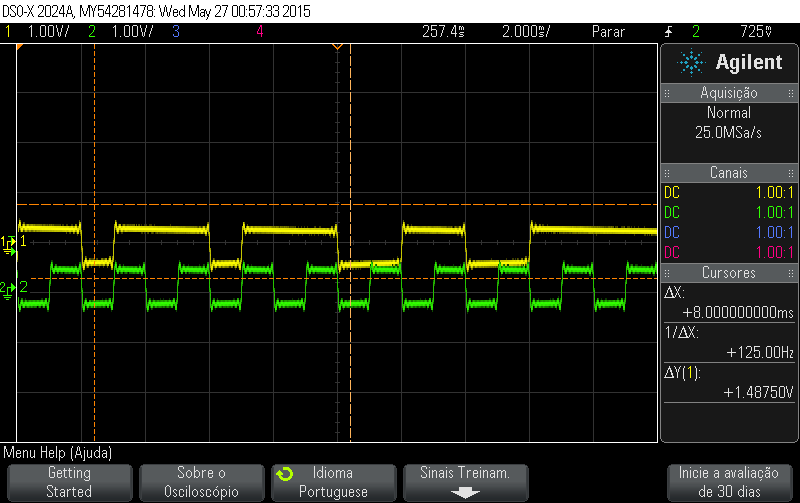
\includegraphics[width=0.6\textwidth]{./en_bn}~\\
	\caption{Visualização da variável en(amarelo) em conjunto com bn(verde).}
	\label{fig:en_bn}
\end{figure}

\begin{figure}[H]
	\centering
	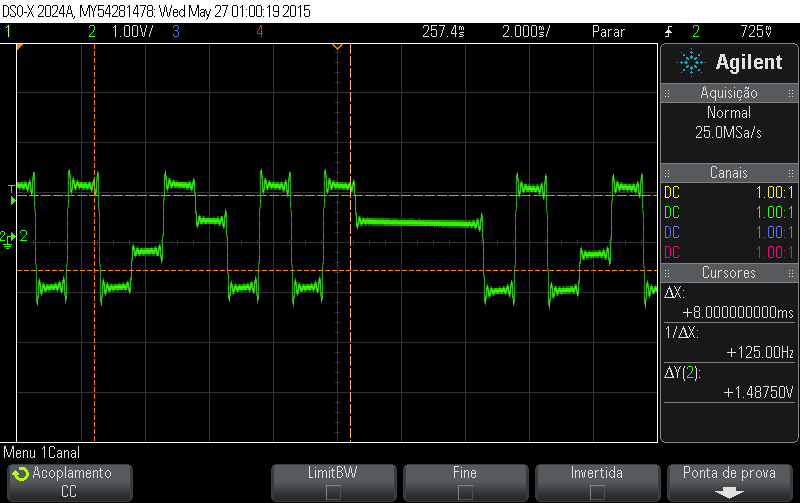
\includegraphics[width=0.6\textwidth]{./scr}~\\
	\caption{Visualização da variável scr.}
	\label{fig:scr}
\end{figure}

Como se pode observar na Figura \ref{fig:en_bn}, é possível criar uma variável pseudo-aleatória a partir de uma variável periódica que varia entre '0' e '1'. As Figuras \ref{fig:en_bn} e \ref{fig:scr} permitem concluir que o \textit{Scrambler} funciona como esperado.

\todo{Ainda tenho de ver o problema da pergunta}

\paragraph{2.Implementação de NCO controlado pelo erro:} \hspace{0pt} \label{para:P3-2}

Para implementar o NCO controlado pelo erro, recorreu-se ao NCO implementado na secção \ref{NCO}, com a mesma rampa, LUT e indexação da mesma como se pode ver no código seguinte.
\begin{lstlisting}
	rampa=rampa+delta;
	index=rampa>>10;
	index=31 & index;
	aux=ampl*LUT[index];aux=aux<<1;
\end{lstlisting}

Mas agora falta a parte de controlar o NCO com o erro. Este controlo da frequência é feito da mesma maneira que na secção \ref{NCO}, através da variável delta (equação \ref{delta}), este controlo observa-se na linha de código a seguir.
\begin{lstlisting}
  delta=16384+(erro>>2);
\end{lstlisting}

Assim, como o erro controla delta e este controla a rampa que indexa a LUT obtém-se um NCO controlado pelo erro.
A seguir prosseguiu-se à obtenção das componentes em fase e em quadratura do sinal pretendido. A componente em fase já tinha sido obtida anteriormente na secção \ref{NCO} pois corresponde ao sinal sinusoidal (figura \ref{quad}). Como a LUT corresponde a meio ciclo do seno foi necessário implementar uma pequena lógica para criar a outra metade do ciclo, enunciada no código a seguir.
\begin{lstlisting}
	if(rampa<0)  seno=-aux>>16;
	else seno=aux>>16;
\end{lstlisting}

Assim, tem-se duas zonas identificadas pelo sinal da rampa, o meio ciclo positivo e o meio ciclo negativo do seno.
No caso da componente em quadratura, devido ao \textit{offset} de 16 amostras obtém-se um sinal coseno. Este não é tão fácil de representar como o seno, desta vez é necessário ter em conta 4 situações, 4 zonas diferentes num ciclo. Nestas zonas o que varia é a secção da LUT que é indexada e o sinal do coseno, que dependem do sinal da rampa e da secção da LUT que estiver a ser indexada para o seno. Estas zonas estão enunciadas nos códigos seguintes.
\vspace{1mm}

\textbf{1ª zona}
\begin{lstlisting}
	if(rampa<0){
	  if(index<=15){
	    aux=ampl*(-LUT[(index+16) & 31]);aux=aux<<1;
	  }coseno=aux>>16;
	}
\end{lstlisting}

A primeira zona do ciclo do coseno corresponde quando a rampa é negativa e o seno está a descer do zero ao seu mínimo (-32767), ou seja, quando se indexa a primeira metade da LUT com o sinal invertido. Assim, quando o seno tem esse comportamento, o coseno está a subir do seu mínimo ao zero, sendo necessário aplicar um \textit{offset} positivo de 16 amostras, ou seja, indexar a segunda metade da LUT, também com o sinal invertido. Foi aplicada uma máscara com 31 de modo ao \textit{offset} nunca causar um índice superior ao permitido na LUT, 31.
\vspace{1mm}

\textbf{2ª zona}

Esta zona também só existe quando a rampa é negativa. No código seguinte pode-se observar o raciocínio implementado para a mesma.
\begin{lstlisting}
	else{
	  aux=ampl*(LUT[(index-16) & 31]); aux=(aux<<1);
	}coseno=aux>>16;
\end{lstlisting}

Continuando o comportamento do seno, este vai subir do mínimo ao zero,ou seja, indexa a segunda metade da LUT mais uma vez com o sinal invertido. Logo, o coseno sobe do zero ao máximo (32767) o que implica um \textit{offset} negativo de 16 amostras para indexar a primeira metade da LUT, sem inverter o sinal.

Para a terceira e quartas zonas efetua-se o mesmo raciocínio de indexação só que só se inverte o sinal da LUT na quarta zona pois nestas a rampa é positiva.
\vspace{1mm}

\textbf{3ª zona}
\begin{lstlisting}
	if(index<=15){
	  aux=ampl*LUT[(index+16) & 31];aux=aux<<1;
	}coseno=aux>>16;
\end{lstlisting}

Aqui, o seno vai subir do zero ao máximo, ou seja, primeira metade da LUT, logo, como o coseno vai descer do máximo ao zero, interessa aceder à segunda metade da LUT, aplicando um \textit{offset} positivo de 16 amostras.
\vspace{1mm}

\textbf{4ª zona}
\begin{lstlisting}
	else{
	  aux=-ampl*LUT[(index-16) & 31];aux=aux<<1;
	}coseno=aux>>16;
\end{lstlisting}

Por fim, chega-se à última zona do ciclo, onde o seno volta ao zero a partir do máximo, ou seja, segunda metade da LUT. Como o coseno volta ao mínimo a partir do zero, aplicando um \textit{offset} negativo de 16 amostras e uma inversão de sinal nas posições indexadas pela LUT.

Assim obteve-se o sinal em quadratura (figura \ref{quad}).
\begin{figure}[h]
	\centering     
	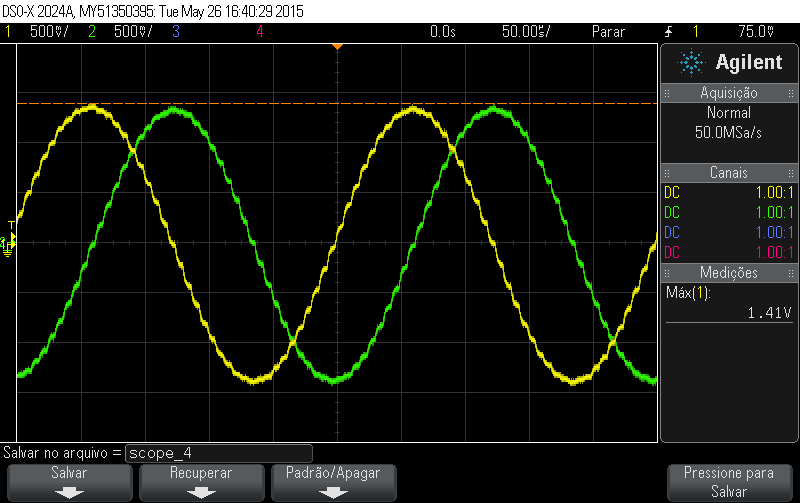
\includegraphics[width=0.6\textwidth]{./quadratura}~\\
	\caption{Componentes e fase(verde) e em quadratura do sinal(amarelo).}
	\label{quad}
\end{figure}

Como se pode observar ao comparar as duas componentes verifica-se qu estão desfasados por um quarto de ciclo, o que significa um offset de 16 amostras.
\paragraph{3.Implementação dos Filtros:} \hspace{0pt}   \label{para:P3-3}       
\todo{guilherme}

O Costas Loop necessita de três filtros passa baixo para o seu correcto funcionamento, sendo dois deles denominados Data Filter e o terceiro Loop Filter.

Os três filtros terão as suas equações às diferenças baseadas na Equação \ref{eq:dif_geral}.

\begin{equation}
y(n)=\alpha y(n-1) + \gamma \frac{1-\alpha}{1-\beta}[x(n)-\beta x(n-1)]
\label{eq:dif_geral}
\end{equation}

Numa primeira fase o valor de $ \beta $ foi considerado '0', ou seja, os filtros teriam apenas um polo. Originando a função de transferência da Equação \ref{eq:tran_geral}.

\begin{equation}
H(z)=\gamma\frac{(1-\alpha)}{1-\alpha z^{-1}}
\label{eq:tran_geral}
\end{equation}

Como queremos filtros com ganho de $ 0dB $ a variável $ \gamma $ das Equações \ref{eq:dif_geral} e \ref{eq:tran_geral} é dimensionada com o valor de '1'. 

Sendo que a equação geral para uma equação às diferenças com o objectivo de implementação está representada na Figura \ref{eq:dif_impl}, podemos concluir que os valores dos coeficientes são os seguintes: $ b_{11}=\alpha $, $ a_{01}=1-\alpha $ e $ a_{11}=0 $.

\begin{equation}
y(n)=b_{11} y(n-1) + a_{01}x(n)-a_{11}x(n-1)
\label{eq:dif_impl}
\end{equation}

Podemos desde já concluir que a representação da saída do filtro pode ser representada no formato dos coeficientes, visto que $ a_{01}+b_{11}=1 $.

Falta apenas calcular a variável $ \alpha $, variável esta que depende da frequência de corte. São então calculados dois valores de $ \alpha $, pois os Data Filter têm um valor de frequência de corte de $ 1kHz $ e o Loop Filter tem um de valor frequência de corte de $ 10Hz $.

Devido à dificuldade do cálculo dos coeficientes caso não aceitássemos aproximações foi decidido utilizar métodos de aproximação. A Equação \ref{eq:alpha} demonstra a fórmula utilizada para calcular uma aproximação de $ \alpha $ em função da frequência de corte.

\begin{equation}
f_{c}=f_{s}\frac{1}{2 \pi}\frac{1-\alpha}{\alpha} \implies \alpha=\frac{f_{s}}{f_{s} + 2 \pi f_{c}}
\label{eq:alpha}
\end{equation}

Utilizando a Equação \ref{eq:alpha} é possível preencher a Tabela \ref{tab:filter_coef} com os valores dos coeficientes.

	\begin{table}[H]
		\centering
		\begin{tabular}{|c|c|c|c|c|c|}
			\hline Filtro & $ f_{c} $ & $ a_{01} $ &  $ b_{11} $ & $ a_{01}|_{Q_{15}} $& $ a_{01}|_{Q_{15}} $ \\ 
			\hline
			\hline Data Filter & $ 1kHz $ & 0.28196980 & 0.71803020 & 9239 & 23528 \\ 
			\hline Loop Filter & $ 10Hz $ & 0.00391163 & 0.99608837 & 128 & 32639 \\ 
			\hline
		\end{tabular}
		\caption{Coeficientes dos filtros e as suas respectivas representações em $ Q_{15} $.}
		\label{tab:filter_coef} 
	\end{table}
	
Os coeficientes da Tabela \ref{tab:filter_coef} podem ser representados em $ Q_{15} $ visto que o módulo de nenhum deles excede '1'.

De seguida segue um excerto código que exemplifica a implementação do Loop Filter. Visto que a implementação dos Data Filter é igual apenas com valores de coeficientes diferentes, não é necessário demonstrar a sua implementação.

\begin{lstlisting}
aux1=(((32639*y)<<1)>>16)	//um shift left para retirar o bit de sinal extra
aux2=(((128*x)<<1)>>16)		//16 shifts rights para se obter um valor de 16 bits em Q15
y=aux1+aux2
\end{lstlisting}

Visto que os filtros têm apenas um polo e nenhum zero, não é necessário recorrer a mais variáveis para guardar valores de entrada ou saída atrasados. A implementação segue a Equação \ref{eq:dif_impl}.

\paragraph{4.\textit{Loop} desmodulador:} \hspace{0pt}
  \todo{rever a linguagem} \label{para:P3-4}

Nesta fase do projeto têm-se todos os blocos necessários do modem BPSK. O sinal de informação $b_n$ foi misturado, $e_n$, codificado e mapeado, $d_n$, e posteriormente multiplicado à portadora com frequência $f_0 = 4kHz$, obtendo o sinal modulado BPSK, $s_n$. Este durante a transmissão pode sofrer variações de fase ($\Delta\phi=\phi_0-\phi_1$) e de frequência ($\Delta f = f_1-f_0$) tomando a forma:
\begin{equation}
	s_n=d_nsin(2\pi f_1t+ \phi_1)
\end{equation}

 Para o desmodular é necessário sincronizar o oscilador local com a frequência da portadora, estimando $\Delta\phi$ e $\Delta f$.

Usa-se, então, o \textit{Costas Loop}, um tipo de PLL. Em semelhança aos seus familiares é composto por um detetor de fase, um \textit{loop filter} e um oscilador local(NCO), excepto nos dois filtros adicionais em cada ramo exterior. No braço inferior o sinal BPSK é multiplicado com o sinal $cos(2\pi f_0t+\phi_0)$ e no superior com $sin(2\pi f_0t+ \phi_0)$ obtendo-se a componente em quadratura e fase do sinal $s_n$, respectivamente: 
\begin{equation}
s_1=\frac{d_n}{2}[cos(4\pi f_0t+\Delta f+\phi_1+\phi_0)+cos(\Delta f+\phi_0-\phi_1)]
\end{equation}
\begin{equation}
s_2=\frac{d_n}{2}[sin(4\pi f_0t+\Delta f+\phi_1+\phi_0)+cos(\Delta f+\phi_0-\phi_1)]
\end{equation} 

Nestes dois multiplicadores ocorre a detecção de fase uma vez que os termos de baixa frequência têm como componentes $\Delta\phi$ e $\Delta f$, os indicadores dos erros de fase e frequência que se usará no NCO. Filtrando-se esses sinais nos \textit{Data filters}, multiplicando-os entre si e passando no \textit{Loop filter} obtém-se 
\begin{equation}
\epsilon(t)=\frac{1}{8}sin(2\Delta\phi)\approx\frac{1}{4}\Delta\phi
\end{equation}

para valores pequenos de $\Delta\phi$. Este sinal estático entra no NCO e aumenta ou diminui a frequência do oscilador reduzindo por consequência o $\Delta f$, desde que a frequência da portadora se encontre na banda de captura do dispositivo descrito.

Uma vez capturada a frequência da portadora (diferente da frequência central) o oscilador local encontra-se sincronizado à frequência da portadora ($f_1 = f_0+\Delta f$) e em fase com a mesma ($\Delta\phi=0$) tendo-se os sinais
\begin{equation}
\frac{1}{2}d_ncos(\Delta\phi)\approx\dfrac{d_n}{2} \hspace{1mm}, \hspace{1mm} \frac{1}{2}d_nsin(\Delta\phi)\approx 0
\end{equation}
à saída do filtro da componente em quadratura e do filtro da componente em fase, respetivamente, tornando-se o braço do primeiro num detetor coerente. Como já mencionado, o espetro do sinal BPSK é o espetro do sinal de informação centrado à frequência da portadora e quando se multiplica pelo sinal local sincronizado obtêm-se réplicas do espetro do sinal de informação a $f=0$ e $f=2f_1$, que ao passar no \textit{Data filter} filtra as componentes superiores a 1kHz obtendo o sinal de informação.


\paragraph{5.Testes do \textit{Costas Loop} com onda sinusoidal} \hspace{0pt} \label{para:P3-5}

Depois de implementar o \textit{Costas Loop} procedeu-se à realização de testes para verificar o seu funcionamento. Primeiro testou-se com uma onda sinusoidal de entrada no \textit{Costas Loop} variando dois parâmetros, a  tensão de pico-a-pico do sinal sinusoidal, V\textsubscript{pp}, a 1V e 3V e a frequência de corte do filtro de \textit{loop}, a 10Hz e a 100Hz. Assim obteve-se quatro situações diferentes com esses parâmetros.

 Estas situações foram criadas primeiro pra testar o braço superior do \textit{Costas Loop} e depois pra testá-lo todo. Para cada situação anotou-se as bandas de captura e de seguimento, observadas através do osciloscópio no sinal do coseno mencionado anteriormente. 
 
 Ao observar o coseno de frequência central 4kHz, constata-se que há uma zona onde o sinal está em sincronismo (figura \ref{cap_segue}a), e para obter a banda de captura analisou-se quando o sinal entra em sincronismo, limite inferior e superior (figura \ref{cap_segue}a).
 
Para a banda de seguimento analisou-se quando o sinal sai do sincronismo, também com os limites inferior e superior (figura \ref{cap_segue}b).
\begin{figure}[h]
	\centering
	\subfloat[]{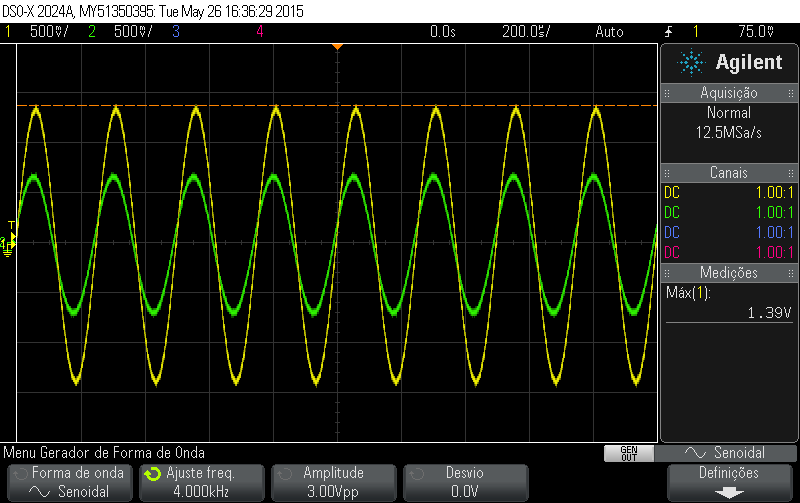
\includegraphics[width=0.4\textwidth]{./captura}}
	\hspace{6 mm}
	\subfloat[]{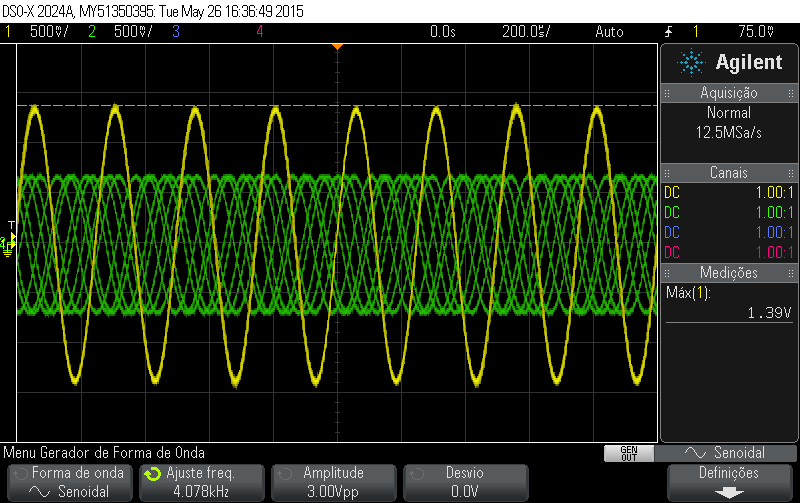
\includegraphics[width=0.4\textwidth]{./segue}}
	\caption{Em sincronismo (a) e fora do sincronismo (b), coseno (verde) e onda sinusoidal (amarelo)}
	\label{cap_segue}
\end{figure}

Ao observar o comportamento do sinal coseno nas figuras, a entrar e a sair do sincronismo, verifica-se que este tem o comportamento de um DPLL clássico.

Para analisar só o braço superior, fez-se com que a entrada do filtro de \textit{loop} fosse o sinal desmodulado, ou seja, ligou-se directamente a saída do filtro de dados à entrada do filtro de \textit{loop}, evidenciado no código seguinte.
\begin{lstlisting}
	s1=((inbuf*coseno)<<1)>>16;
	y1=(((23528*y1)<<1)>>16)+(((9239*s1)<<1)>>16);
	s=y1; //braco superior
\end{lstlisting}

Antes de proceder aos resultados das bandas é necessário salientar que ao considerar um filtro de \textit{loop} de 100 Hz foi necessário calcular os coeficientes do filtro de novo. No código a seguir observa-se os dois filtros implementados e a diferença nos seus coeficientes. 
\begin{lstlisting}
	erro = (((32639*erro)<<1)>>16)+(((128*s)<<1)>>16); //10Hz
	//erro= (((31529*erro)<<1)>>16)+(((1238*s)<<1)>>16);//100Hz
\end{lstlisting}

Assim, podem-se observar as bandas resultantes do braço superior nas tabelas seguintes.
\begin{figure}[H]
	\centering
	\subfloat[]{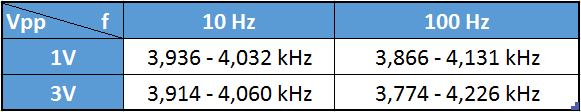
\includegraphics[width=0.45\textwidth]{./tabela_cap}}
	\hspace{6 mm}
	\subfloat[]{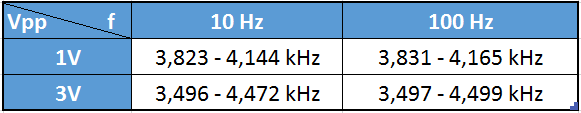
\includegraphics[width=0.45\textwidth]{./tabela_segue}}
\end{figure}

A tabela (a) corresponde às bandas de captura e a tabela (b) corresponde às bandas de seguimento. Como se pode ver, todas as bandas compreendem a frequência 4 kHz, oscilando sempre em relação à mesma.
É possível também constatar que ao aumentar a amplitude da onda sinusoidal ou a frequência de corte do filtro \textit{loop} a banda de captura aumenta, principalmente com a frequência de corte do filtro. No caso da banda de seguimento só a amplitude é que aumenta a mesma.

Passando ao teste do \textit{Costas Loop} inteiro, é necessário contabilizar o braço inferior na entrada do filtro de \textit{loop} através da linha de código a seguir.
\begin{lstlisting}
	s2=((inbuf*seno)<<1)>>16;
	y2=(((23528*y2)<<1)>>16)+(((9239*s2)<<1)>>16);
	s=((y1*y2)<<1)>>16; //y2 e o braco inferior
\end{lstlisting}

Pode-se observar os resultados na tabela seguinte, desta vez considerou-se apenas uma situação. 
\begin{figure}[H]
	\centering
	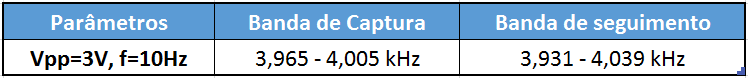
\includegraphics[width=0.65\textwidth]{./tab_costa}~\\
\end{figure}

Comparativamente ao braço superior, ambas as bandas reduziram significativamente com a adição do braço inferior.

\paragraph{6.Testes do \textit{Costas Loop} com BPSK sem zero nos filtros} \hspace{0pt} \label{para:P3-6}

Depois de efetuados os testes com a onda sinusoidal passou-se ao objetivo deste projeto e testou-se o \textit{Costas Loop} usando como entrada o sinal modulado do transmissor BPSK desenvolvido na secção \ref{p2}. Como tal foi necessário alterar o código para as entradas dos filtros de dados.
\begin{lstlisting}
	s1=((sn*coseno)<<1)>>16; //sn e o sinal modulado
	s2=((sn*seno)<<1)>>16;
\end{lstlisting}
Depois de feitas as alterações recorreu-se ao osciloscópio para analisar o sinal desmodulado, s, (figura \ref{demod_sz}) para poder comparar com o sinal $d_n$. O objetivo é o sinal desmodulado ser o mais próximo possível de $d_n$ pois este foi o sinal modulado no transmissor BPSK.
\begin{figure}[H]
 	\centering
 	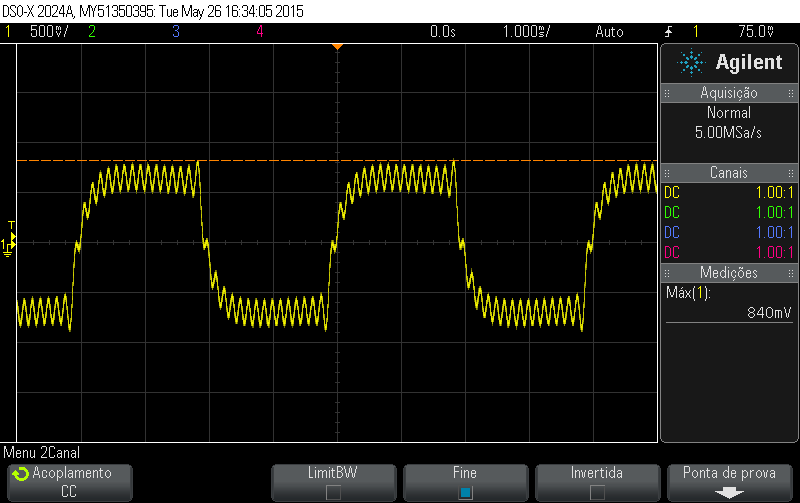
\includegraphics[width=0.6\textwidth]{./demod_semzero}~\\
 	\caption{Sinal desmodulado}
 	\label{demod_sz}
\end{figure}
É possível observar alguma semelhança a $d_n$ como uma onda quadrada, mas esta contém uma distorção substancial no sinal, distorção essa que teve de ser tratada para poder analisar e testar o \textit{Costas Loop} como deve ser. Este tratamento e a razão pela qual é necessário são explicados na secção seguinte.
\paragraph{7.Testes do \textit{Costas Loop} com BPSK com zero nos filtros} \hspace{0pt} \label{para:P3-7}

O sinal obtido do \textit{Costas Loop} ainda apresenta um vestígio da multiplicação no detetor de fase, sendo possível observar-se uma oscilação de maior frequência somada ao sinal de informação. Tal é devido ao aliasing existente nos filtros discretos que, dadas as réplicas espectrais somarem o ganho no limite de Nyquist, $\frac{F_s}{2} = 8kHz$, o filtro  não é seletivo que chegue a essa frequência, resultando no observado na figura acima. Posto isto, optou-se por eliminar este ruído da maneira mais simples possível: inserir um zero na função de transferência dos filtros de dados à frequência do sinal de ruído. Para tal utilizou-se a equação às diferenças do enunciado, como na alínea P.3, e determinou-se a função de transferência:
\begin{equation}
H(z) = \gamma\frac{1-\alpha}{1-\beta}\dfrac{1-\beta z^{-1}}{1-\alpha z^{-1}}
\end{equation}

O ganho estático ($\gamma$) foi obtido igualando a função a 1 à frequência $\omega=0 => z=1$. O valor de $\alpha$ foi determinado na alínea P.3 e o valor de $\beta$ foi determinado igualando a função transferência a 0 à frequência $z=e^{j\omega T_s}|_{\omega=2\pi8000}$. Desta maneira insere-se um \textit{Notch} para os 8kHz obtendo-se um \textit{Lowpass Notch filter} com a frequência de corte de 1kHz na mesma contudo com uma atenuação muito maior à frequência do sinal ruído.
A equação às diferenças toma então a forma:
\begin{equation}
y_n = \alpha y_{n-1}+\gamma\frac{1-\alpha}{1-\beta}(x_n-\beta x_{n-1}), 
\end{equation}
com $\beta=-1; \alpha=0.7180302; \gamma=1.$

No programa alterou-se apenas os valores dos coeficientes da equação às diferenças dos \textit{data filters}.

\begin{lstlisting}
y1= (((23528*y1)<<1)>>16)+(((4620*s1_0)<<1)>>16)+(((4620*s1_1)<<1)>>16);

y2=(((23528*y2)<<1)>>16)+(((4620*s2_0)<<1)>>16)+(((4620*s2_1)<<1)>>16);
\end{lstlisting}
Observa-se na figura abaixo o sinal desmodulado sem o ruído e o sinal de informação.

\begin{figure}[H]
	\centering
	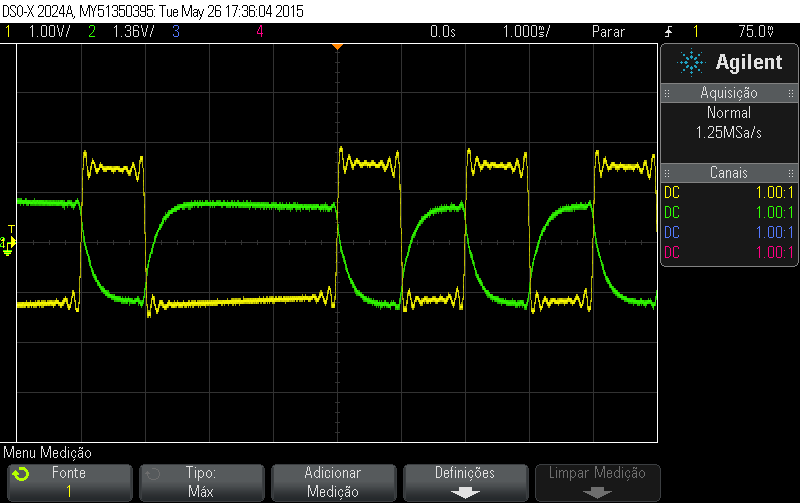
\includegraphics[width=0.5\textwidth]{./dn_y1}~\\
	\caption{sinal de informação, $d_n$,(amarelo) e sinal desmodulado(verde).}
	\label{demod}
\end{figure}

De seguida observa-se como previsto que, uma vez que nos encontramos em sincronismo com o transmissor os sinais resultantes dos detetores de fase, $s_1$ e $s_2$ são a onda de informação com uma componente de alta frequência somada e zero, respetivamente.

\begin{figure}[H]
	\centering
	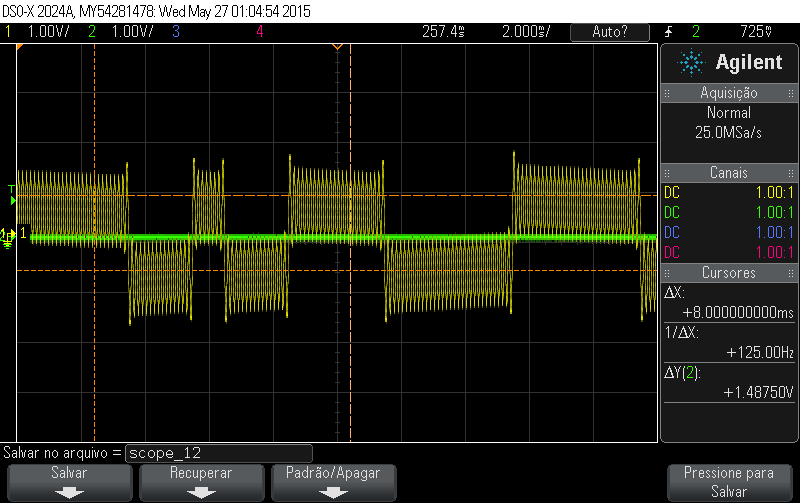
\includegraphics[width=0.5\textwidth]{./s1_s2n}~\\
	\caption{sinal de quadratura, $s_1$,(amarelo) e sinal de fase, $s_2$(verde).}
	\label{s1_s2}
\end{figure}

Agora tem-se uma ilustração do sinal de erro com o sinal desmodulado. O primeiro como previsto, mais uma vez porque o \textit{Costas Loop} está sincronizado, é nulo pois não se tem $\Delta\phi$ e $\Delta f$.

\begin{figure}[H]
	\centering
	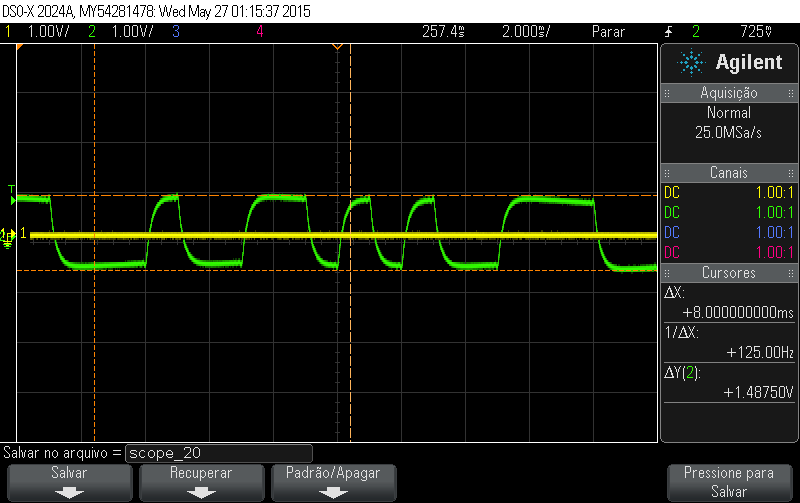
\includegraphics[width=0.5\textwidth]{./erro_y1n}~\\
	\caption{sinal de erro, $\epsilon$,(amarelo) e sinal desmodulado (verde).}
	\label{erro_y1n}
\end{figure}

Por fim representa-se os outputs dos data filters e o espetro do sinal desmodulado.

\begin{figure}[H]
	\centering
	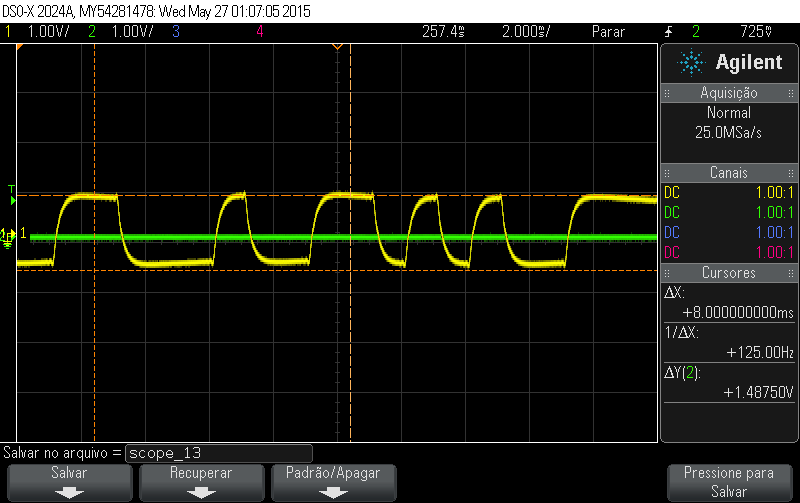
\includegraphics[width=0.5\textwidth]{./y1_y2n}~\\
	\caption{saída do filtro de quadratura(amarelo) e saída do filtro de fase(verde).}
	\label{y1_y2n}
\end{figure}

\begin{figure}[H]
	\centering
	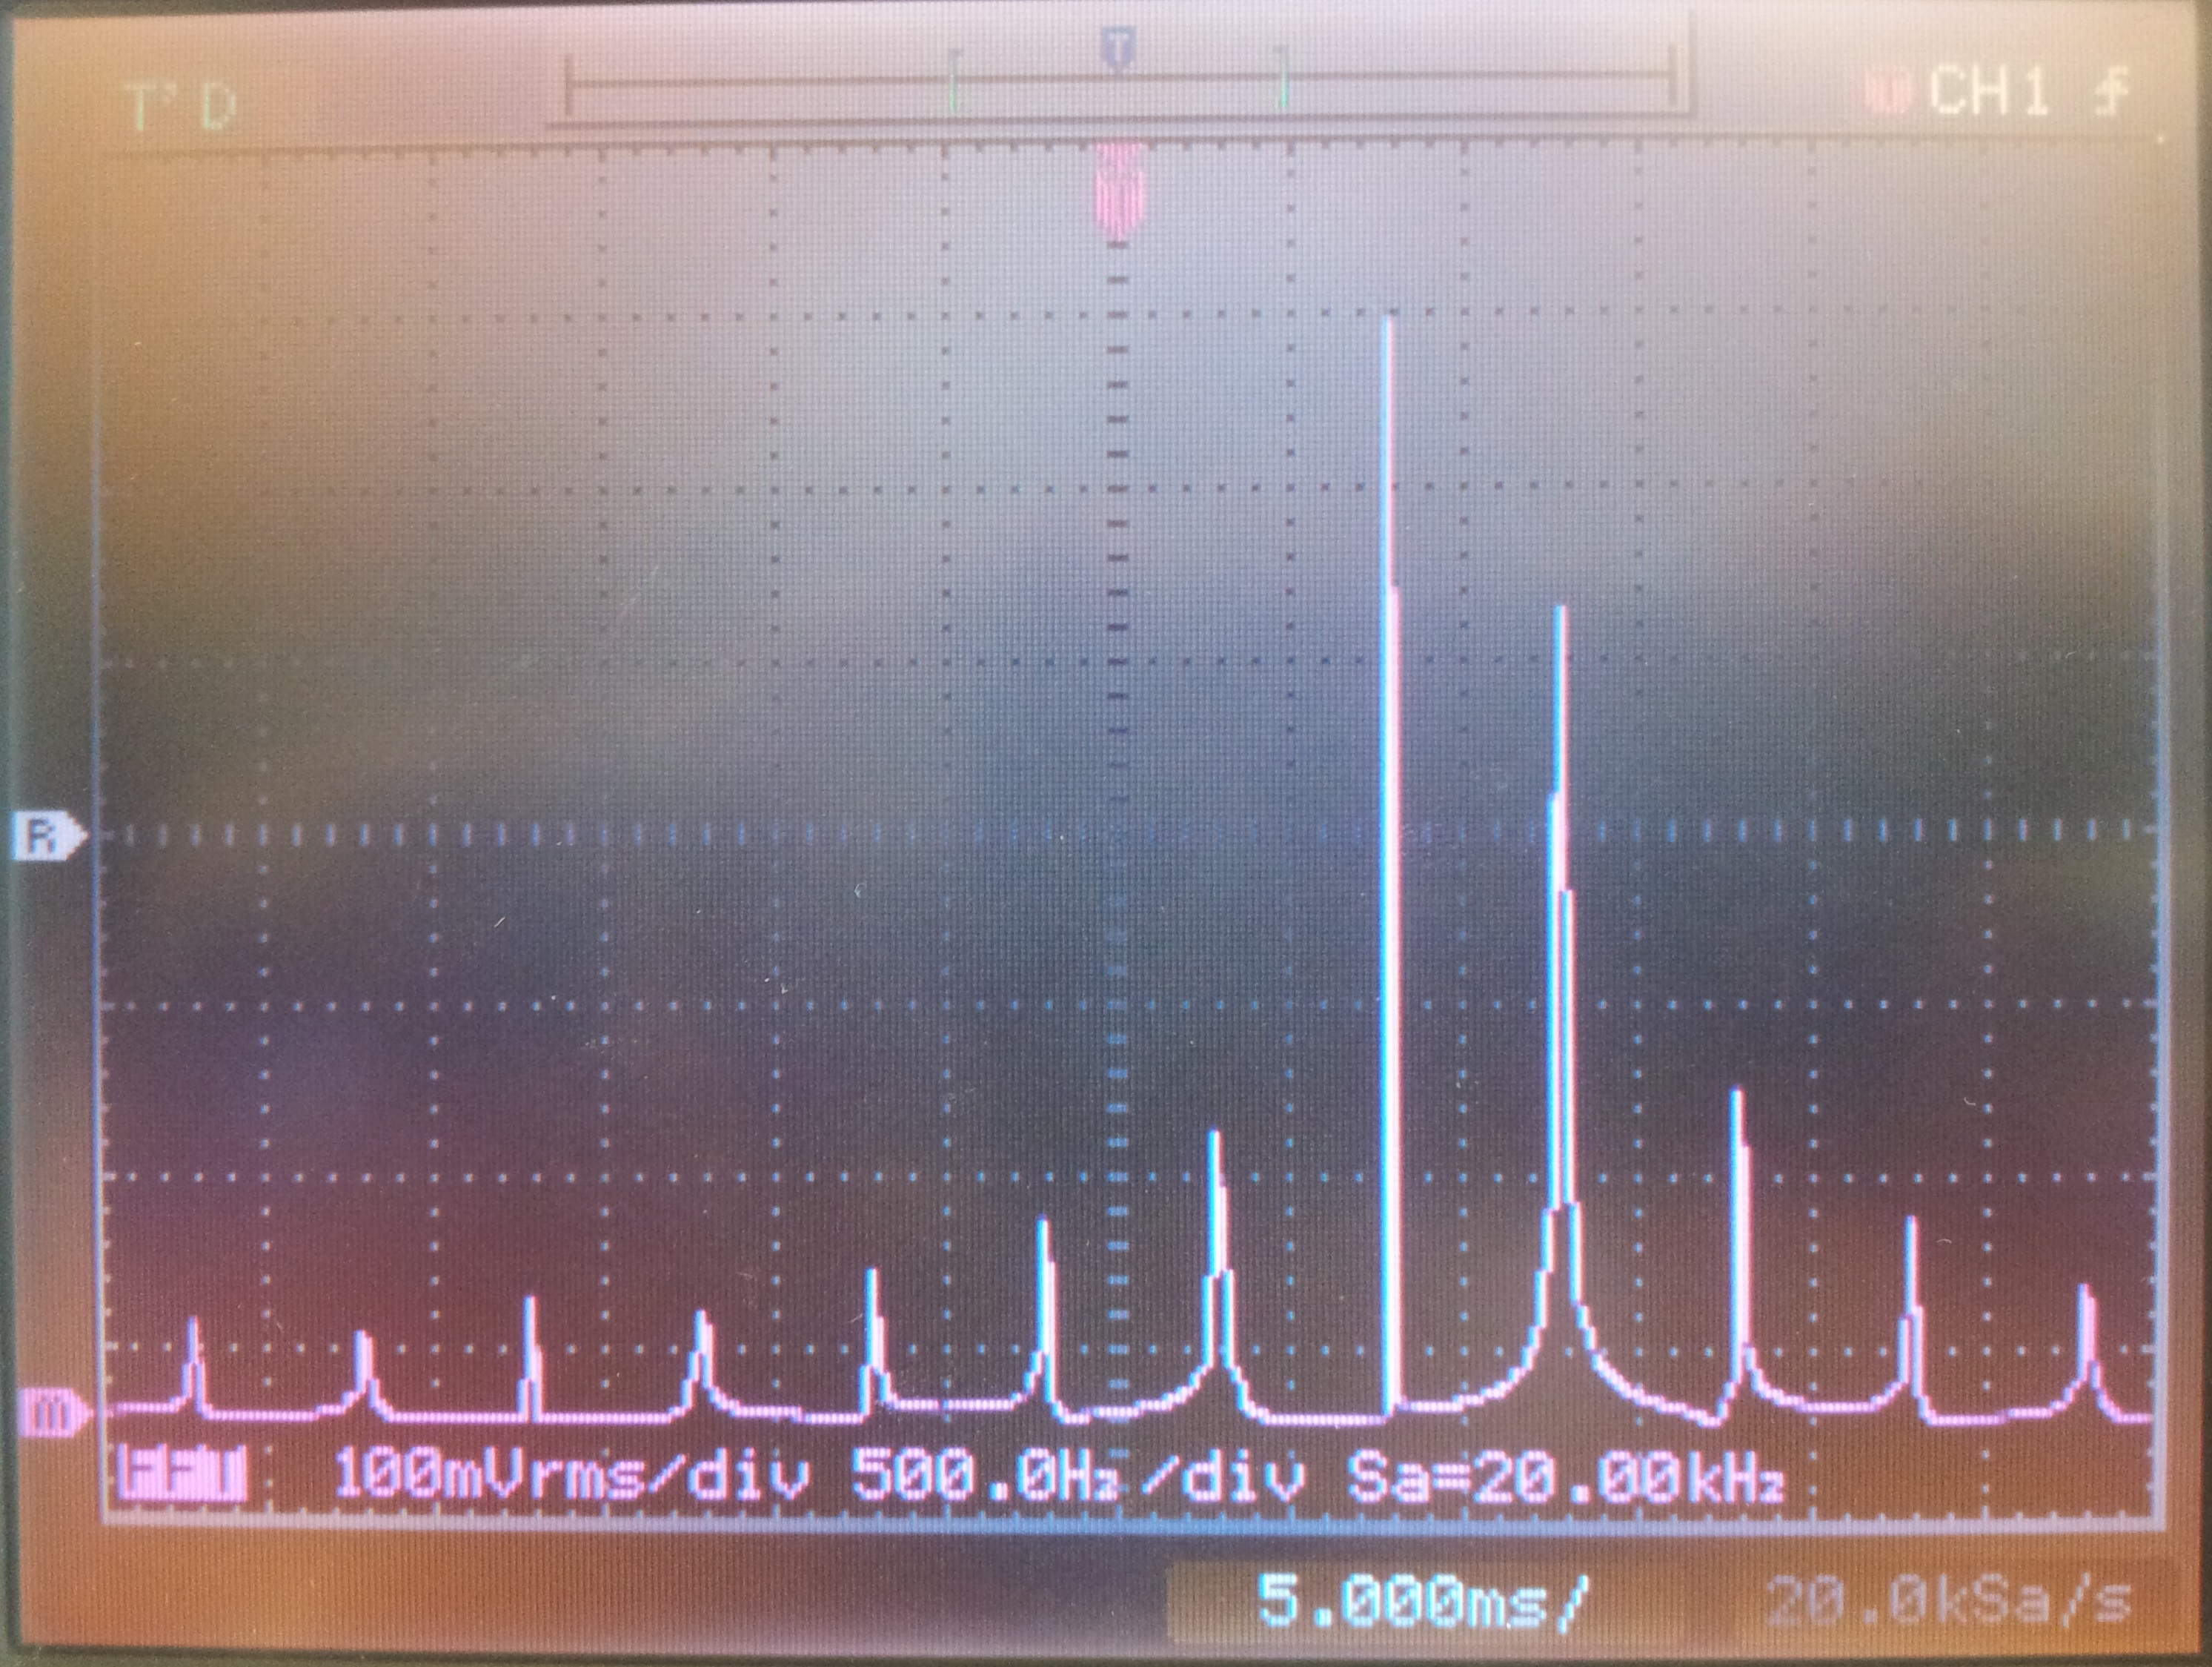
\includegraphics[width=0.5\textwidth]{./espetro}~\\
	\caption{Espetro do sinal desmodulado.}
	\label{espetro}
\end{figure}

Como se pode observar, o espetro trata-se de um $sinc$, com zeros nos múltiplos pares da frequência de $d_n$, $f_d=\frac{f_bit}{2}$, com a escala horizontal com 1kHz/divisão.

\paragraph{8.Transient} \hspace{0pt} \label{para:P3-8}

De forma a se poder observar o transitório de aquisição do \textit{Costas Loop}, com a finalidade de poder analisar características adicionais do mesmo, nomeadamente o tempo para se obter sincronismo, fez-se uma análise \textit{transient}. Esta consiste em induzir no circuito um erro de fase elevado, uma vez que é mais simples a alterar a frequência do sinal BPSK, saturando a cada 4000 amostras o valor da variável do erro ( $\epsilon=$ 32767). Observa-se na figura seguinte os sinais de erro e a saìda desmodulada, para um \textit{Loop filter} com frequência de corte, $f_c = 10Hz$:

\begin{figure}[H]
	\centering
	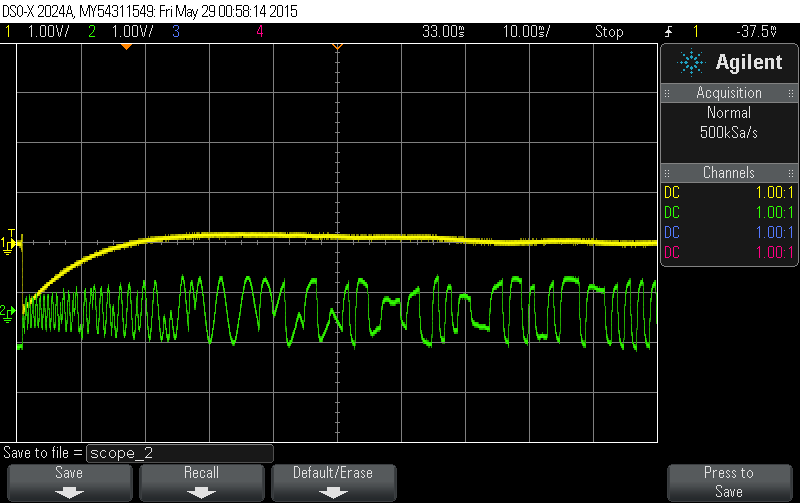
\includegraphics[width=0.5\textwidth]{./transient10Hz}~\\
	\caption{sinal de erro, $\epsilon$, (amarelo) e sinal desmodulado(verde).}
	\label{trans10}
\end{figure}
Observa-se o comportamento esperado do erro com algum overshoot, um curto tempo de estabelecimento e convergindo para 0. Ao mesmo tempo a forma de onda assemelha-se cada vez mais com o sinal de informação. Para este caso tem-se um tempo de sincronismo de $\sim$53ms, tendo em conta a escala horizontal ter 10ms/divisão.

Repetiu-se este teste para um \textit{Loop filter} com frequência de corte, $f_c = 100Hz$, e verificou-se que este circuito sincroniza mais rapidamente com um tempo de sincronismo de $\sim$10ms, tal como se observa na figura seguinte, com a mesma escala horizontal do caso anterior.

\begin{figure}[H]
	\centering
	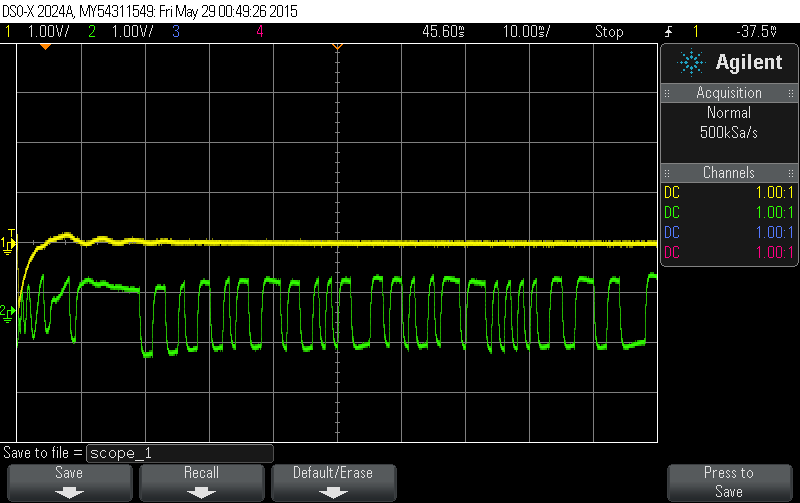
\includegraphics[width=0.5\textwidth]{./transient100Hz}~\\
	\caption{sinal de erro, $\epsilon$, (amarelo) e sinal desmodulado(verde).}
	\label{trans100}
\end{figure}


\section{Conclusão}

\todo{alterar conclusao}

No projeto do oscilador, aprendeu-se como controlar um oscilador a partir de vários parâmetros e o efeito de interpolação linear no mesmo. Como já foi afirmado, a interpolação criou um sinal com maior precisão embora não tenha sido possível observar essa melhoria devido às limitações do equipamento utilizado.

No projeto do transmissor criou-se a primeira parte do modem BPSK, aproveitando o conhecimento adquirido no projeto do oscilador, e observou-se os efeitos da modulação de uma sequência de bits codificada e mapeada, tanto no tempo como na frequência, o que deu para observar pelas inversões de fase presentes no sinal modulado e nas harmónicas do espetro.

\section{Anexos}
\todo{acrescentar codigo da parte 2}
\subsection{Anexo A}
Oscilador Controlado Numericamente:
\lstinputlisting[language=C]{bpsk.c}

\subsection{Anexo B}
Transmissor BPSK:
\lstinputlisting[language=C]{transmissor.c}

\subsection{Anexo C}
BPSK Modem:
\lstinputlisting[language=C]{final.c}

\end{document}